\documentclass[11pt]{article}
\usepackage{amsmath}
\usepackage{amsfonts}
\usepackage[]{graphicx}
\usepackage{subfig}
\usepackage[utf8]{inputenc}
\usepackage{float} % for forcing latex to put images nearby they are called
\usepackage{amsmath}
\usepackage{amsfonts}
\usepackage{cite}
\usepackage{amssymb}
\usepackage[]{graphicx}
\usepackage{hyperref}
\usepackage{xcolor}
\usepackage{natbib}
%\usepackage{draftwatermark}
%\SetWatermarkText{DRAFT}
%\SetWatermarkScale{5}
\usepackage[printwatermark]{xwatermark}
\usepackage{tikz}
\usepackage{pifont}
%\usepackage{capt-of}
%\usepackage{tabu}
\usepackage{subfig}
\begin{document}
%\maketitle

\begin{figure}[ht]
\centering
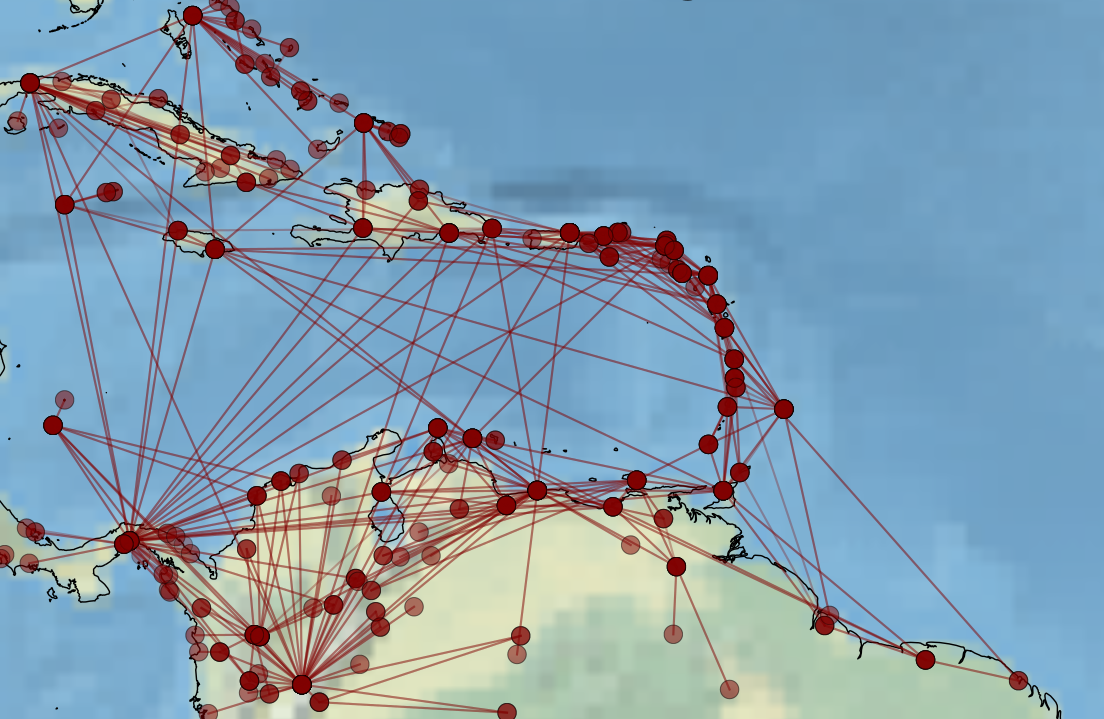
\includegraphics[scale=.17]{./caribbean_region}
\hspace{.35cm}
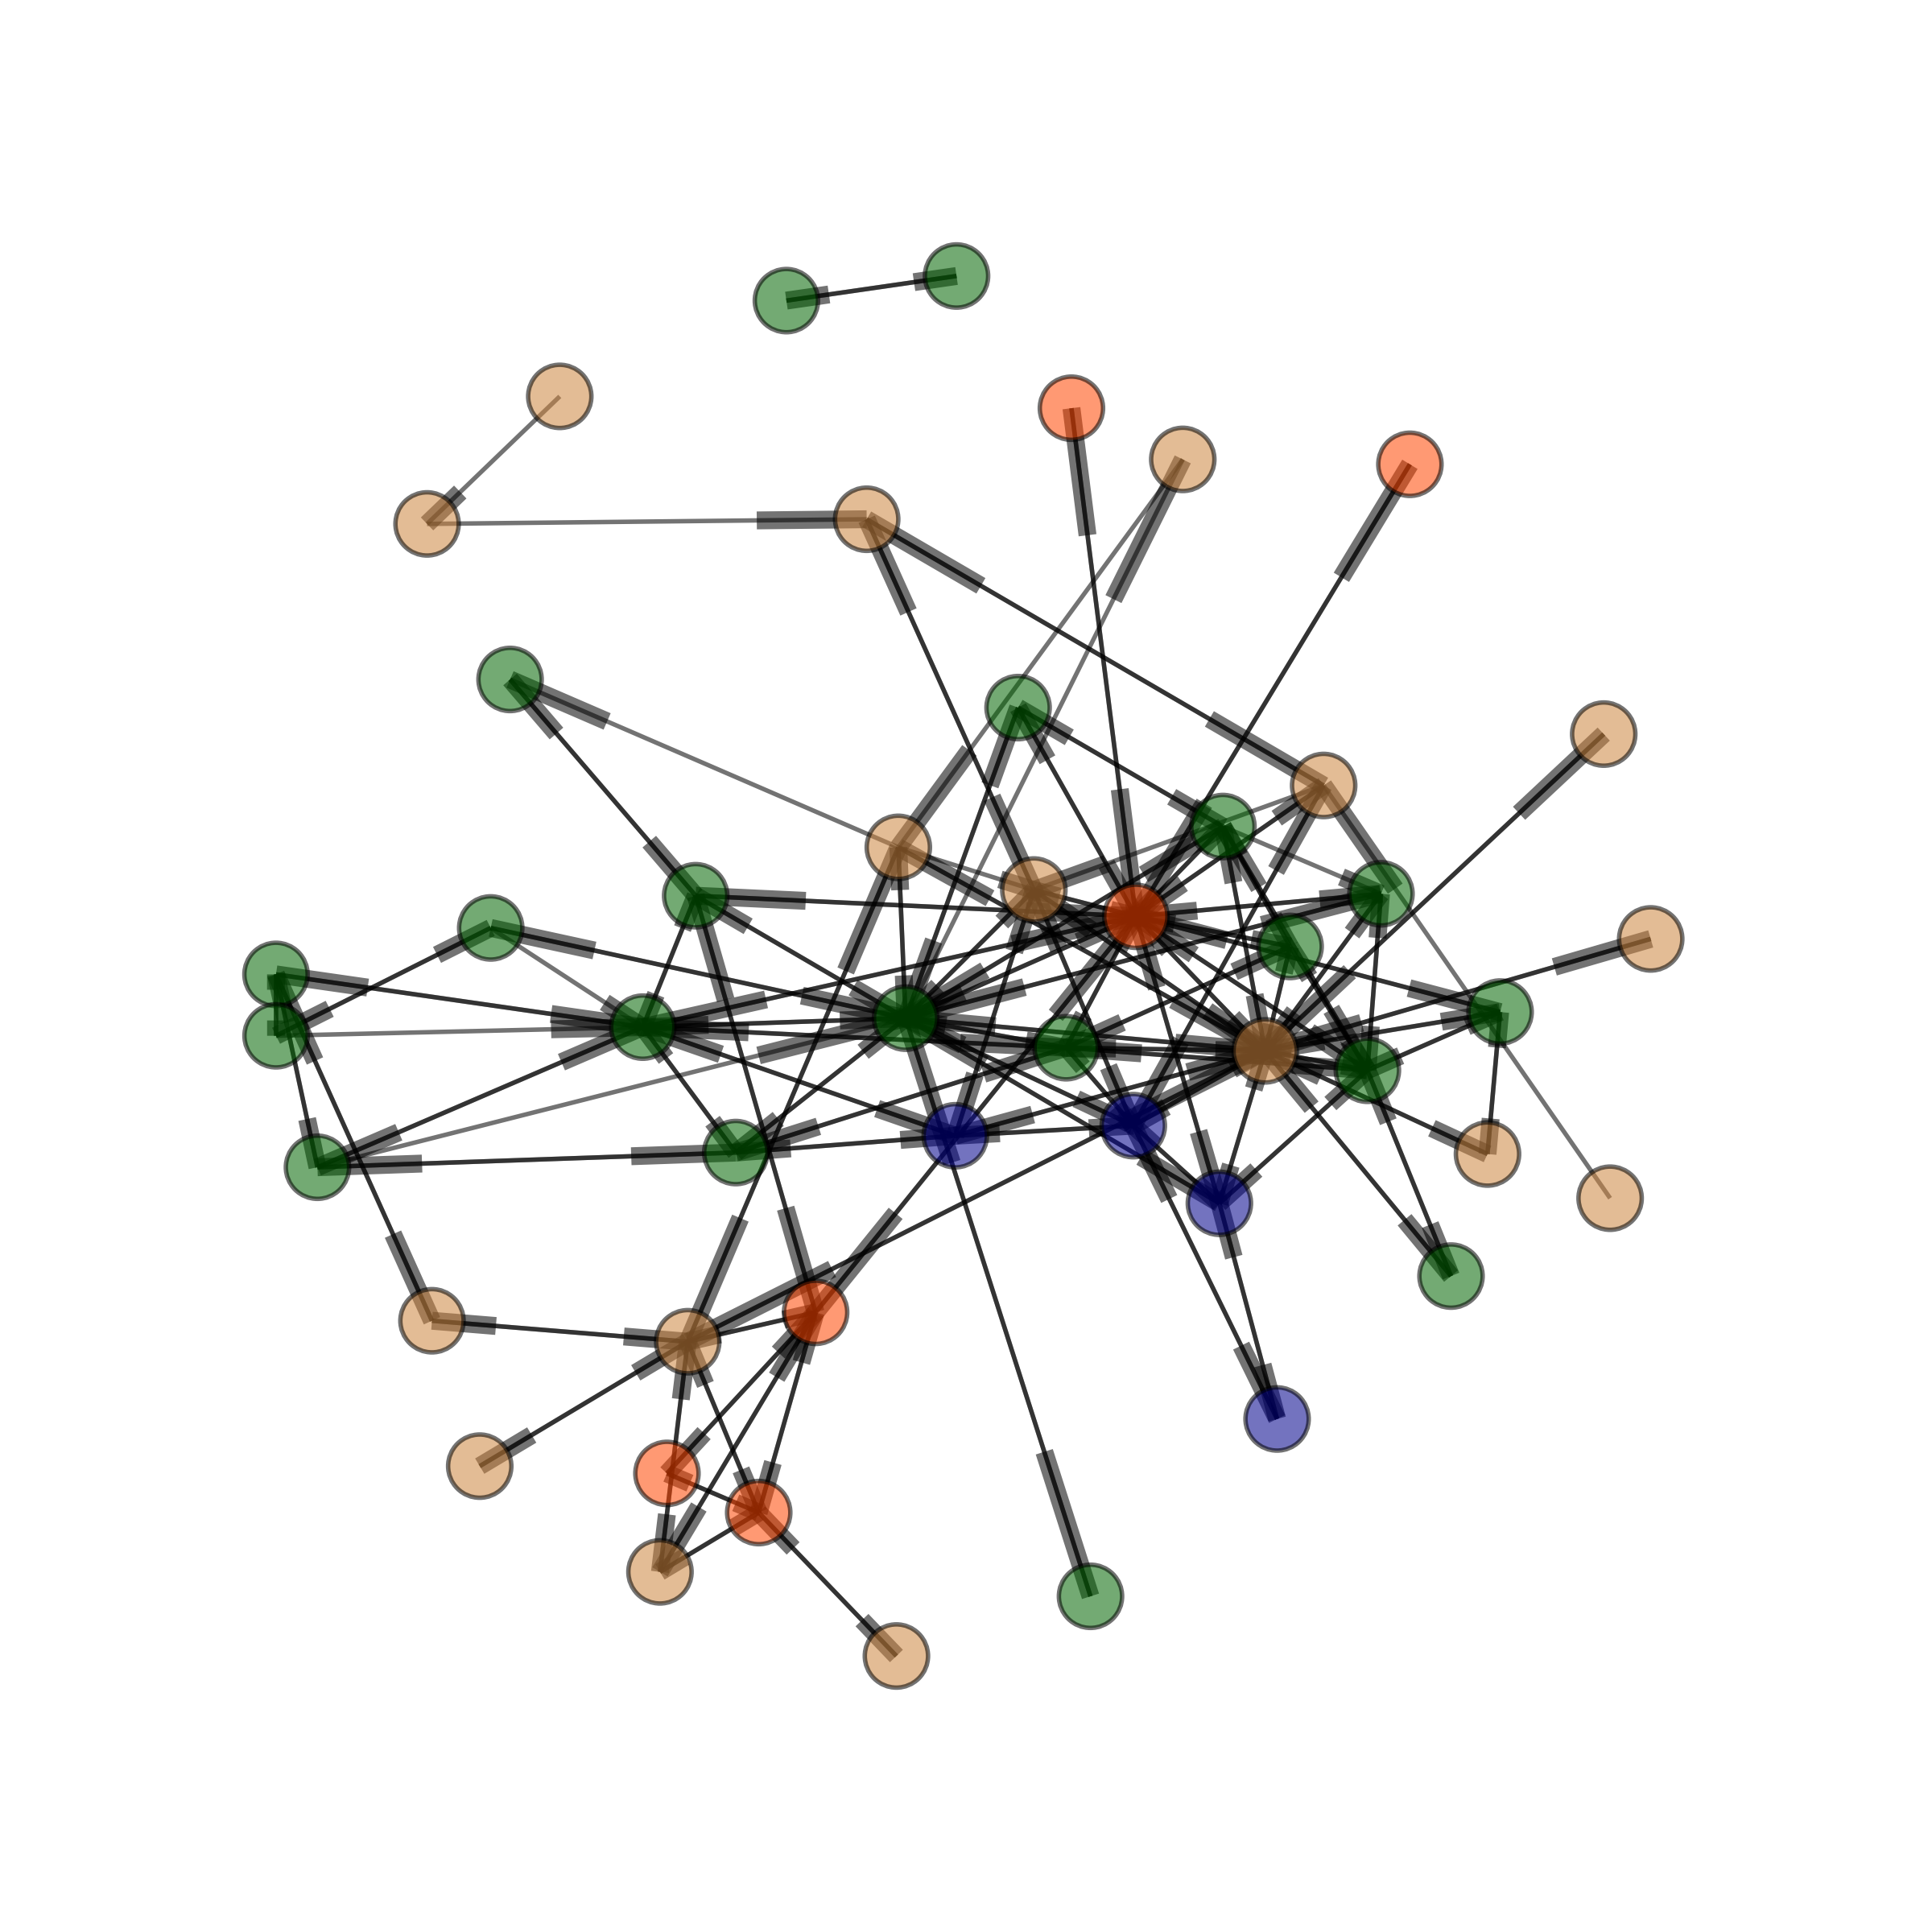
\includegraphics[scale=.33]{./graph_region3_colored}
%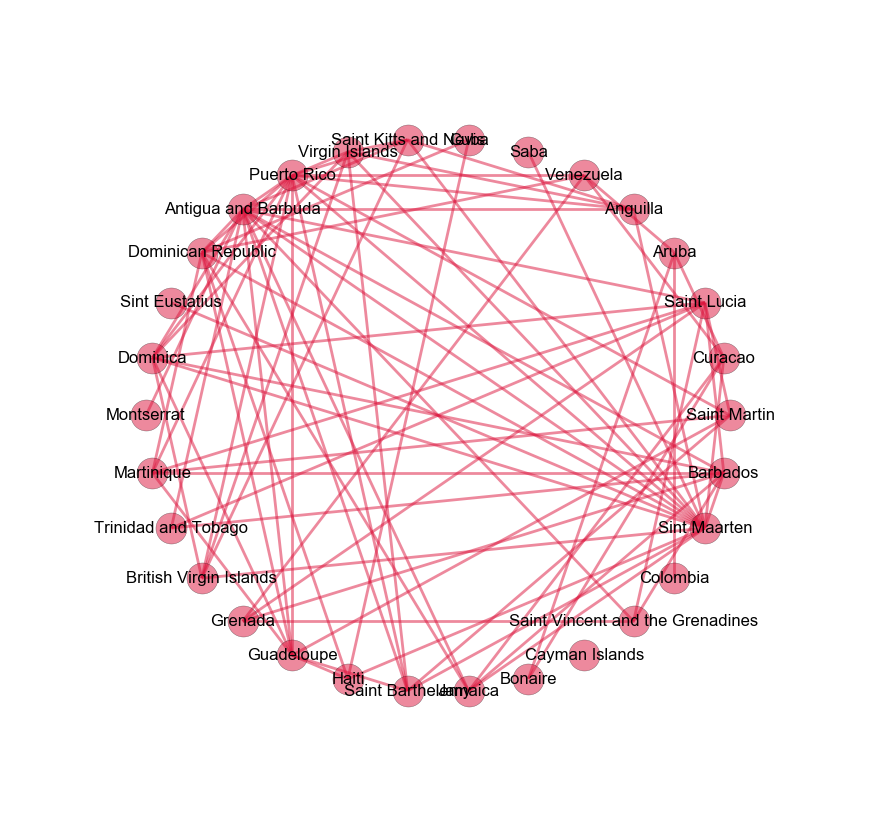
\includegraphics[scale=.16]{./simple_network_model_circular_and_labels_red_scen_A}\\
\caption{\small Modeled region and model network based on commercial airline traffic during the years 2013-2014 (www.openflights.com).}
\label{fig:map-and-network}
\end{figure}

%\vspace{2cm}

\begin{figure}[ht]
\centering
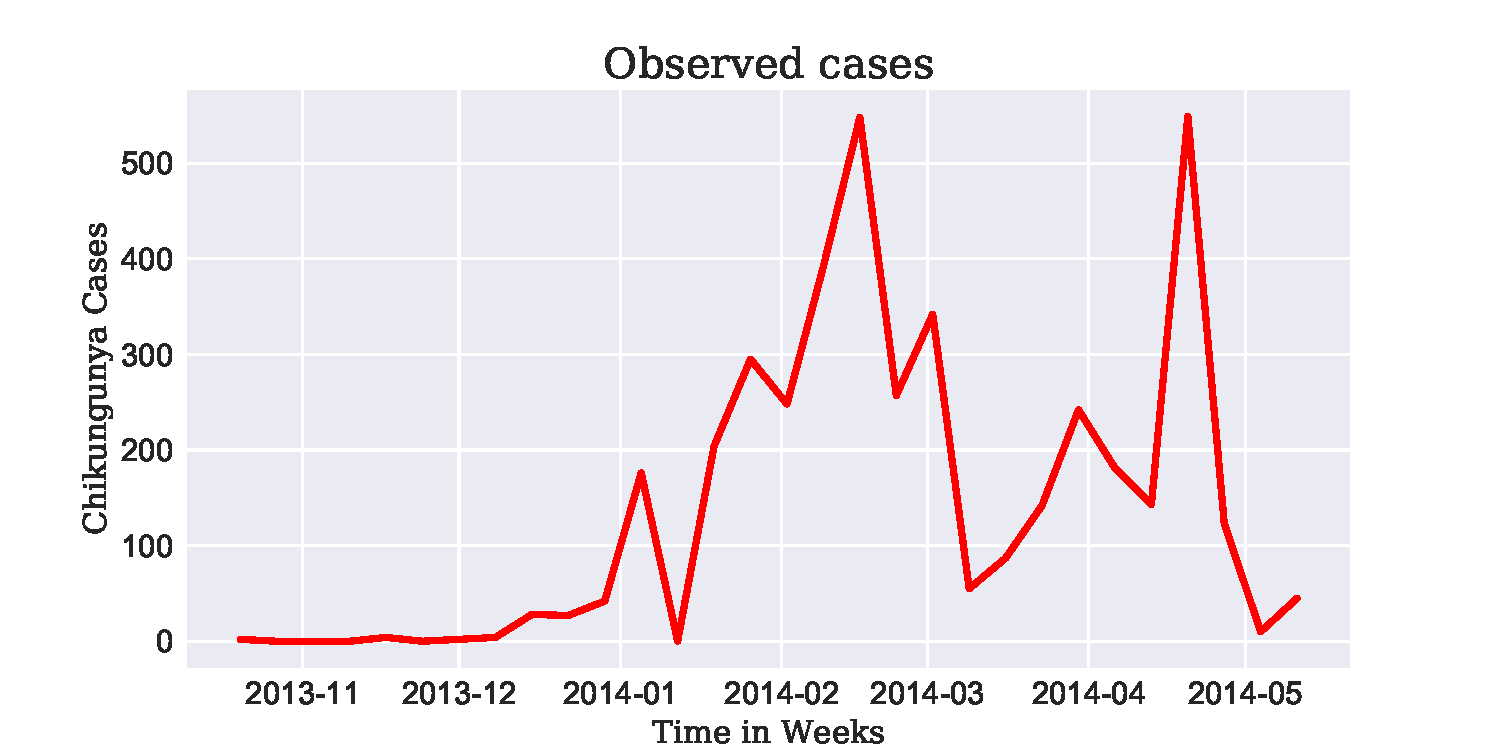
\includegraphics[scale=.24]{./observed_cases_st}
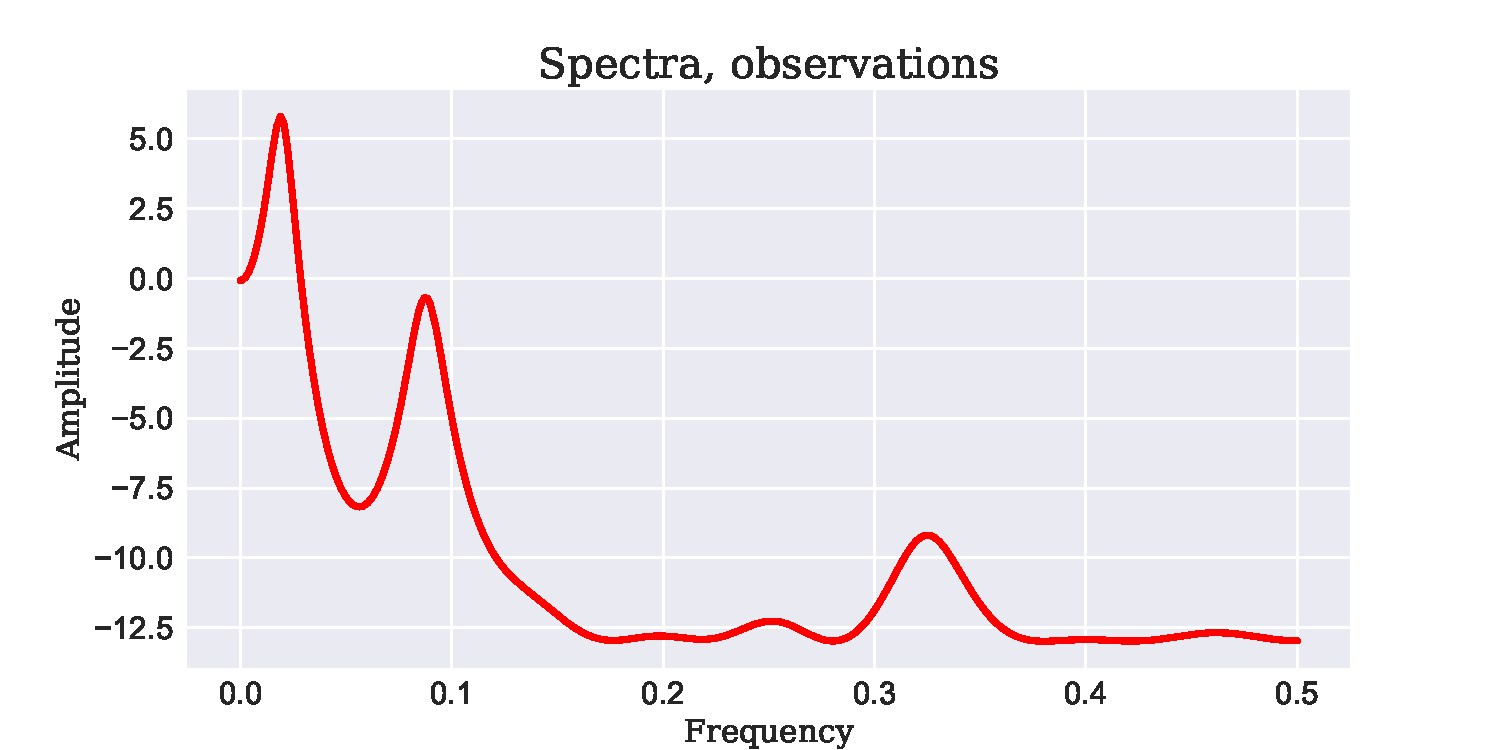
\includegraphics[scale=.24]{./spectra_obs}
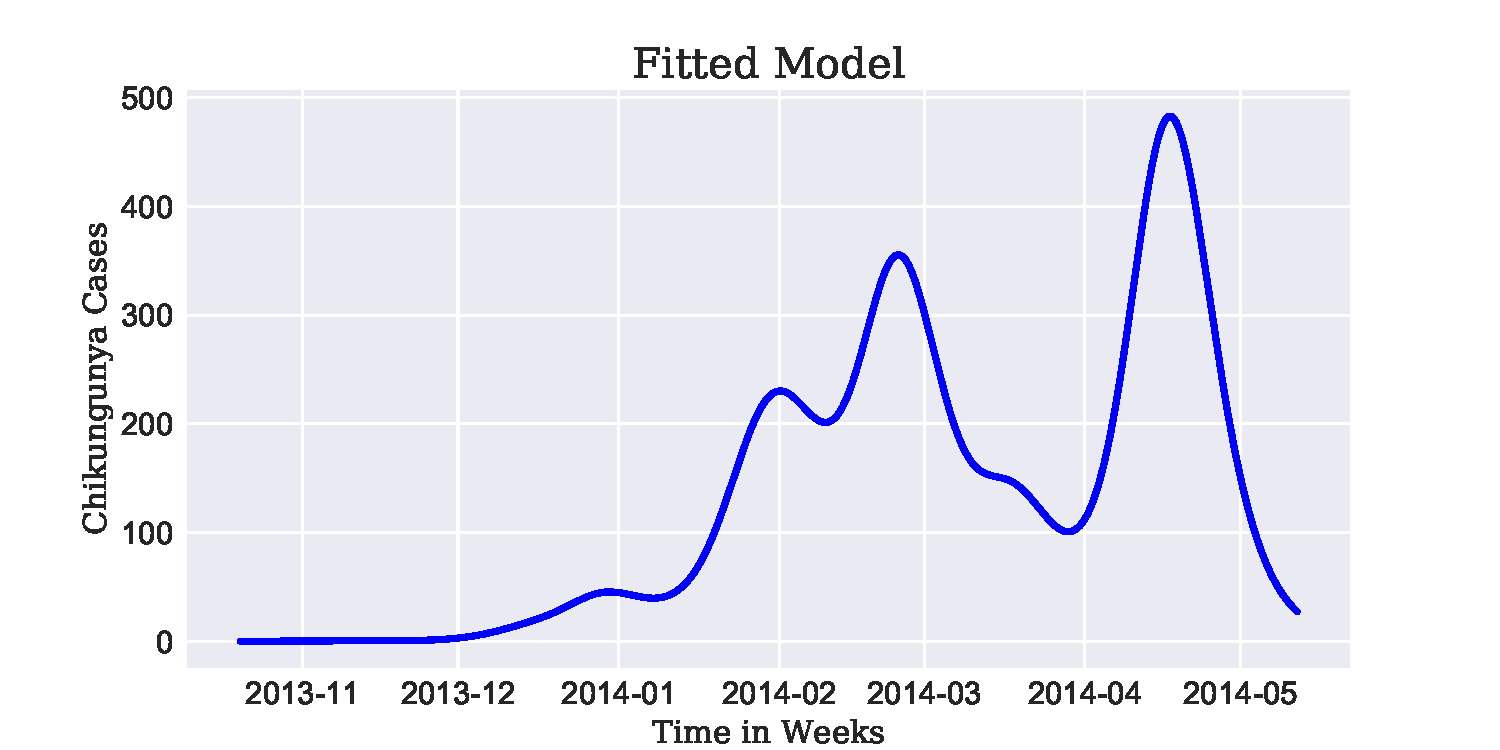
\includegraphics[scale=.24]{./fitted_model_st}
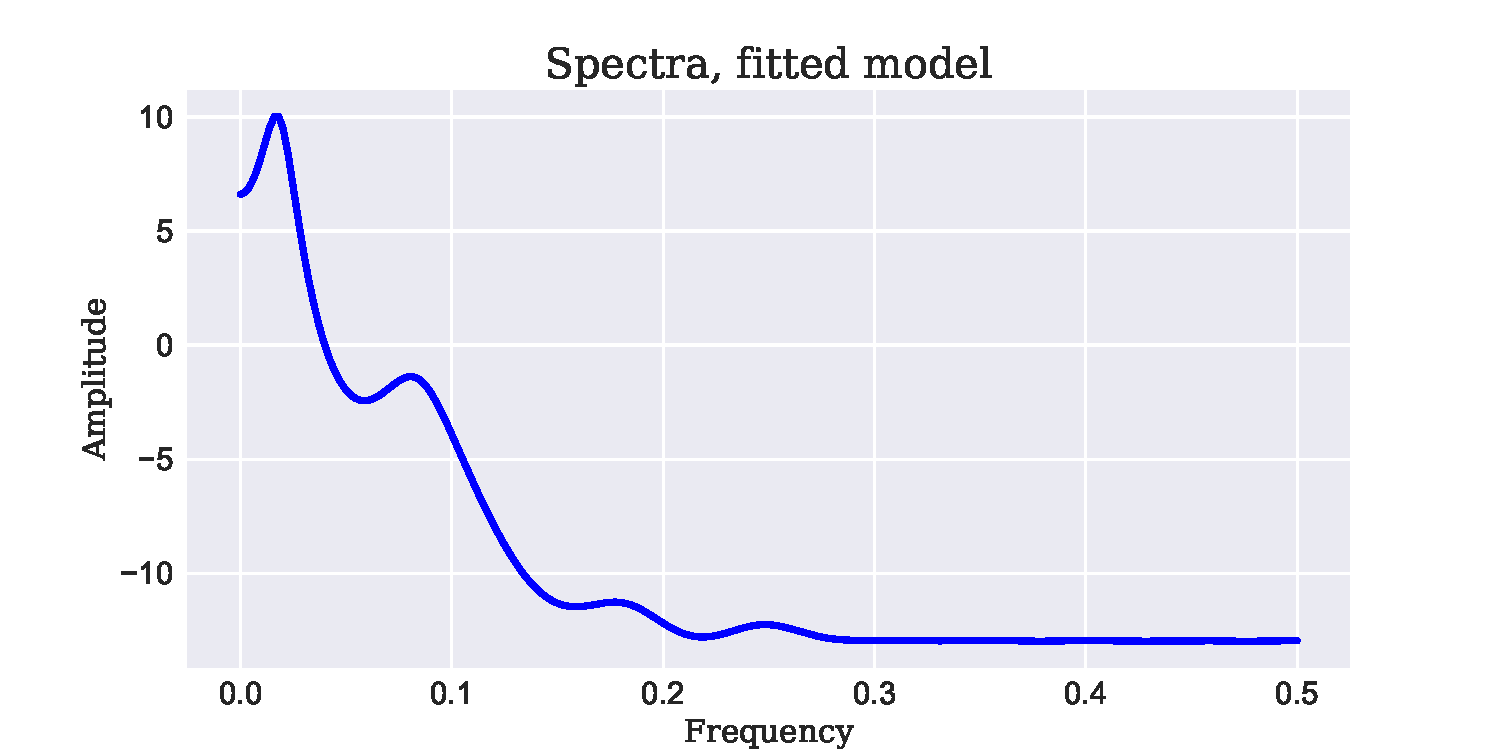
\includegraphics[scale=.24]{./spectra_sim}\\
\caption{\small Aggregated reported chikungunya cases of the first 300 days of the outbreak and spectra of the observed time series (left up and bottom respectively); fitted (aggreagated) solution of the network-SEIR model and spectra of the solution (right up and bottom respectively).}
\label{fig:data-model-spectra}
\end{figure}

\vspace{2cm}

\begin{figure}[ht]
\centering
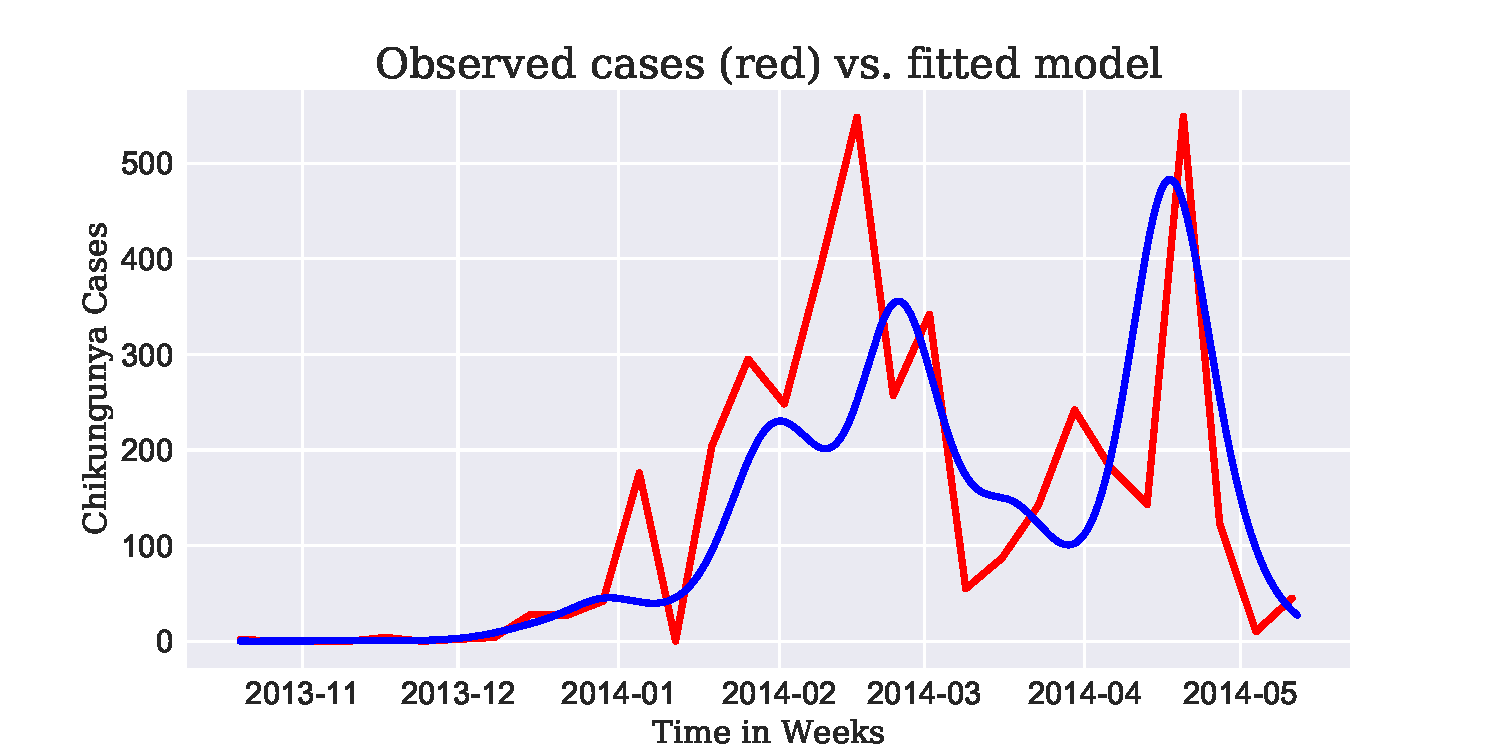
\includegraphics[scale=.24]{./observed_vs_fitted_st}
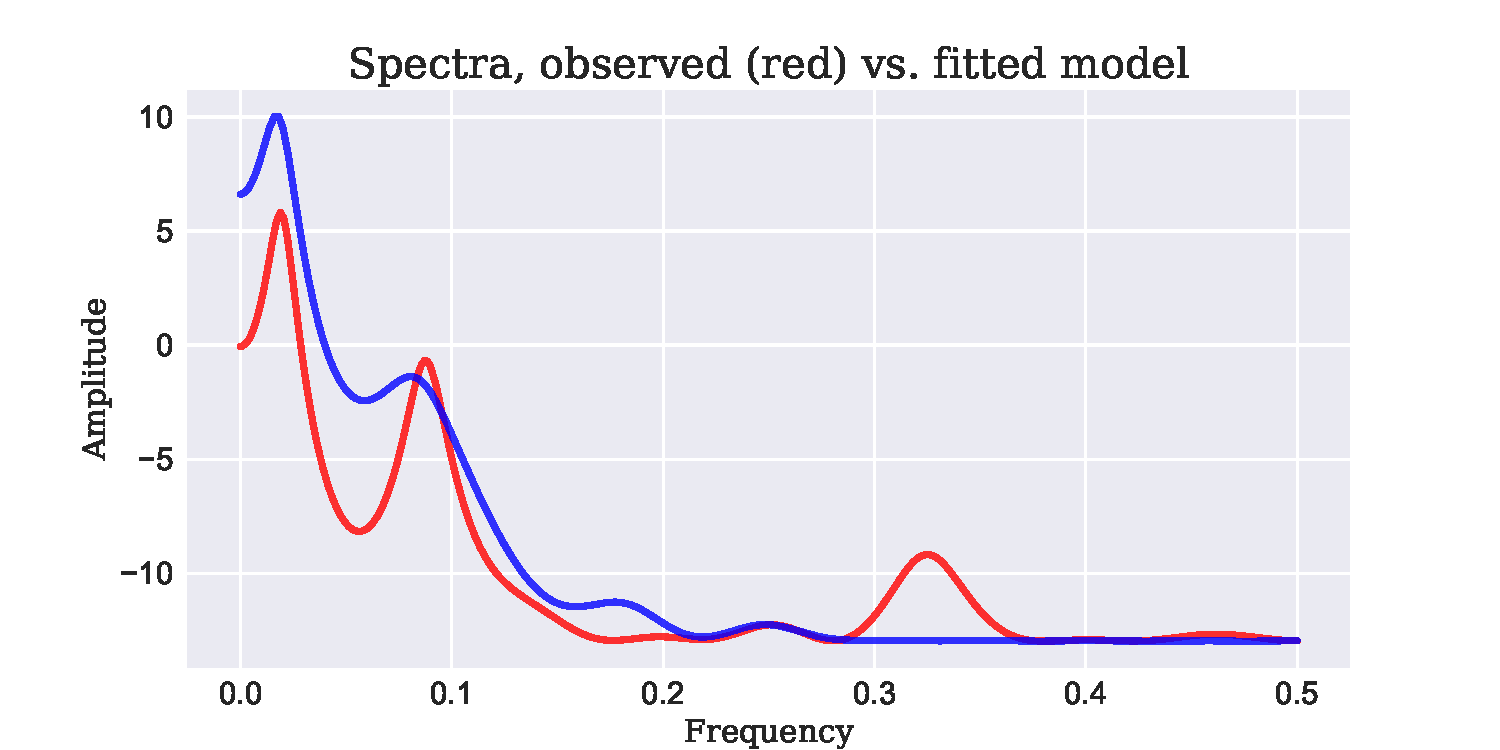
\includegraphics[scale=.24]{./spectra_obs_vs_sim}
\caption{\small (Alternative) In the left pannel we show aggregated reported chikungunya cases of the first 300 days of the outbreak (red) and fitted (aggreagated) solution of the network-SEIR models (blue).  Right pannel is the spectra of the observed time series (red)  and the spectra of the fitted network-SEIR aggregated solution.}
\label{fig:data-model-spectra-alt}
\end{figure}

\vspace{4cm}

\begin{figure}[ht]
\centering
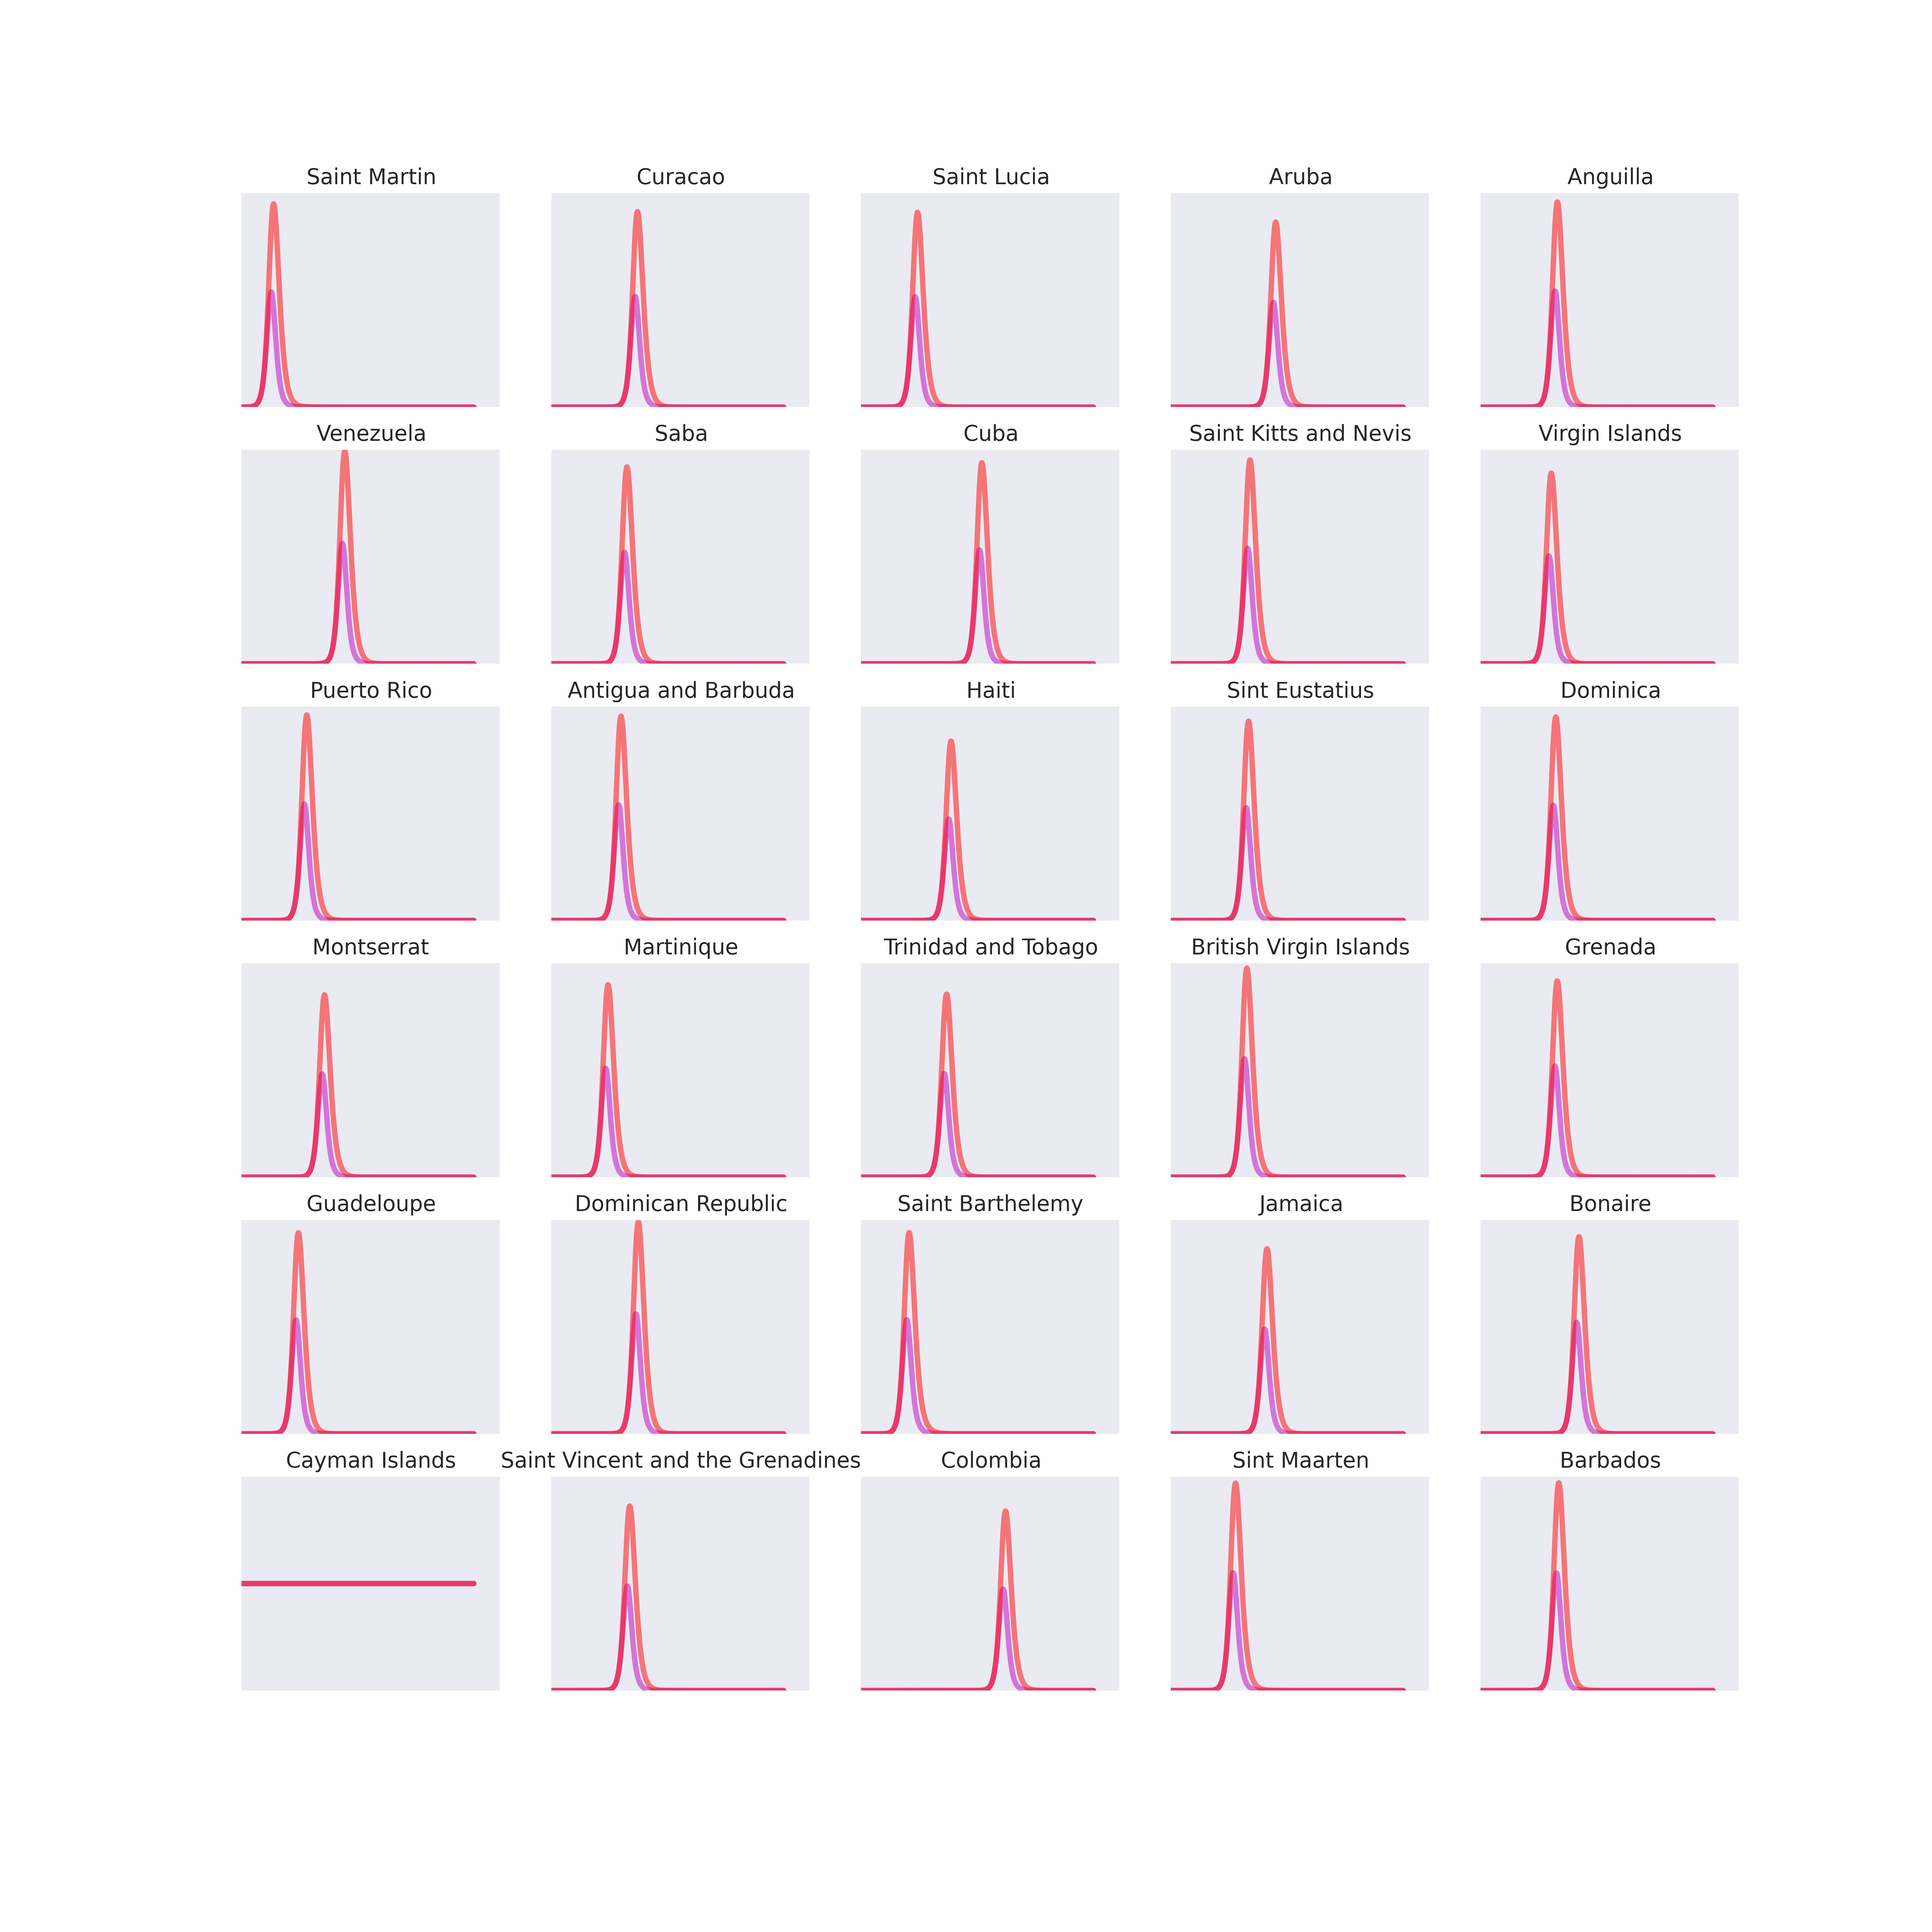
\includegraphics[scale=.06]{./wave}
\caption{\small Epidemic wave. The profile of the solutions of the network-SEIR model is shown here for each individual nodes. The curves with larger amplitude correspond to simulated exposed individuals whereas the smaller amplitudes correspond to infected individuals.}
\label{fig:wave}
\end{figure}


\vspace{4cm}

\begin{figure}[ht]
\centering
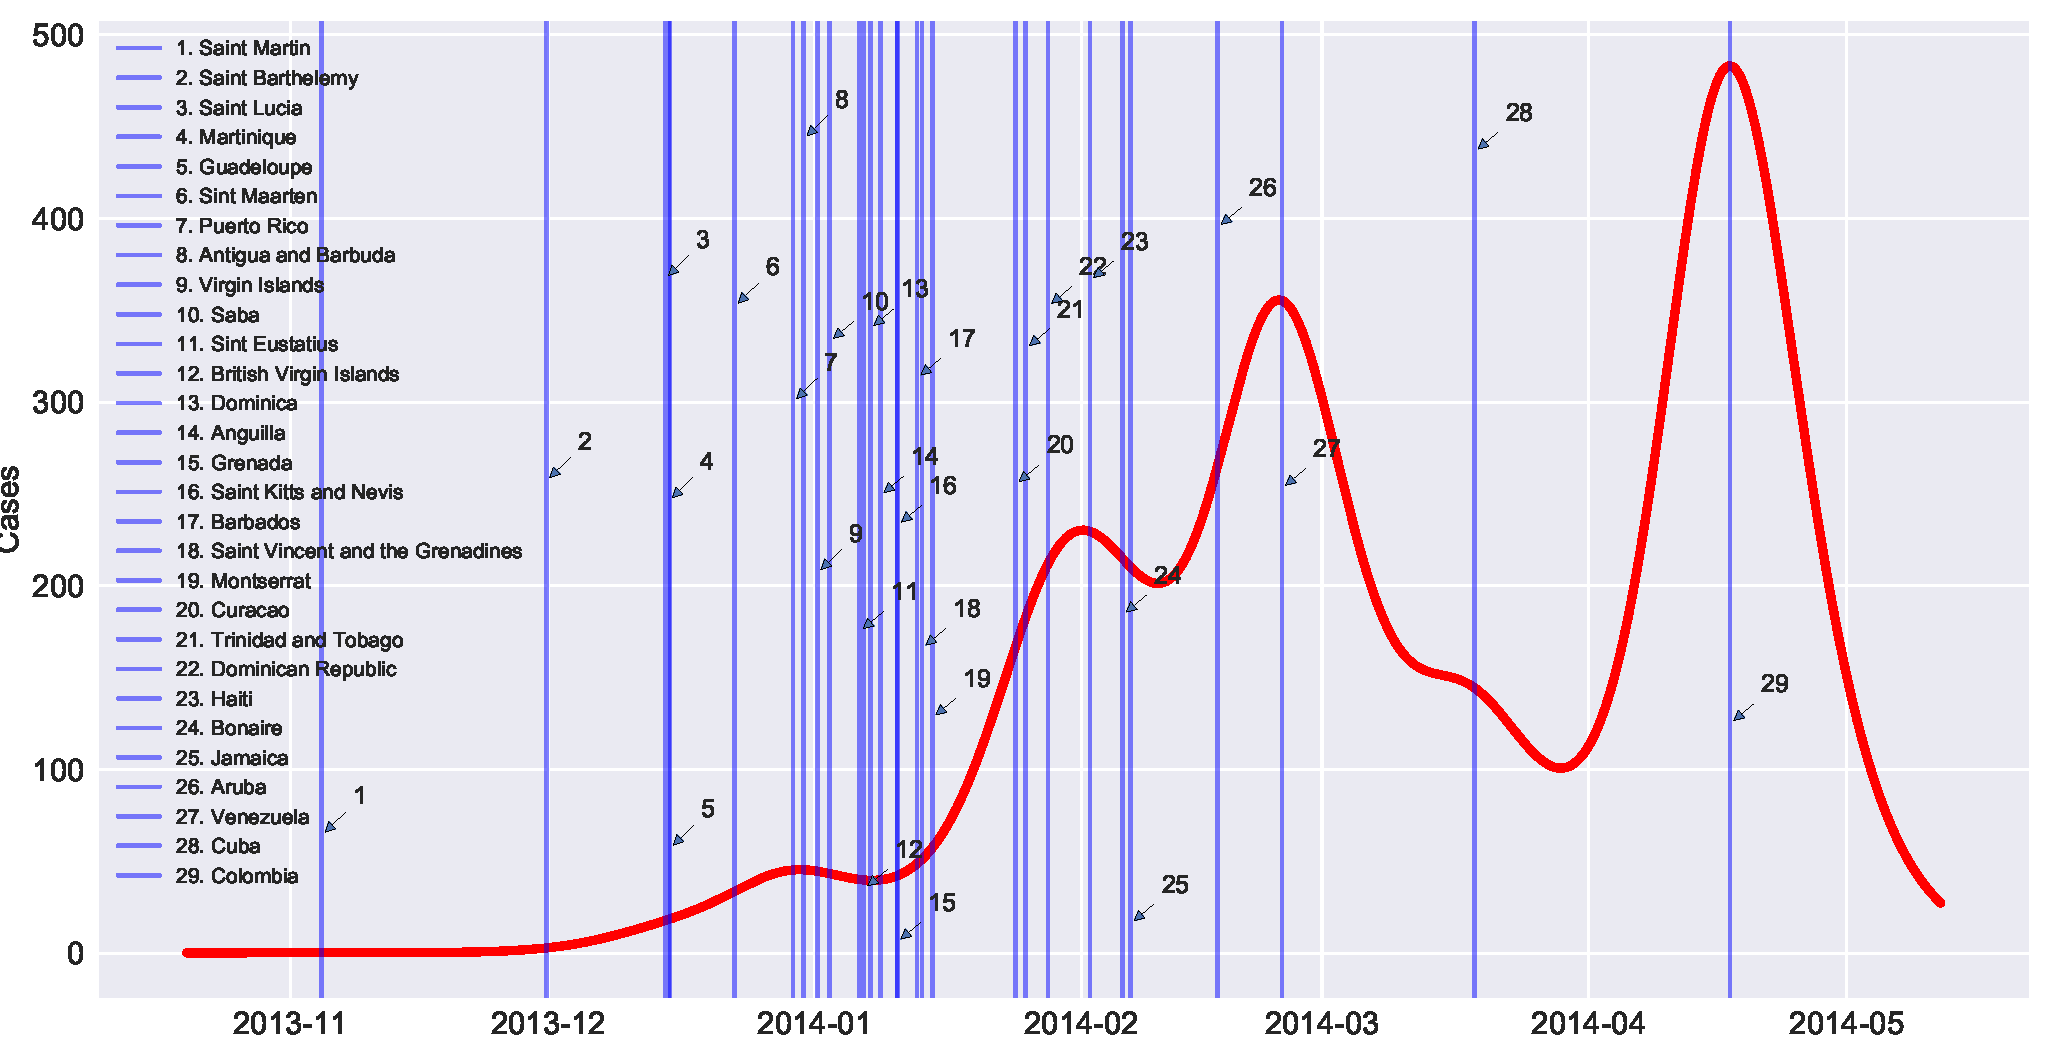
\includegraphics[scale=.38]{./wave4}
\caption{\small Epidemic wave. The vertical blue lines indicate the maxima epidemic peak for each local network node/location. The legend in the left indicate the order as the appear in the models. The red line is the aggregated model solution.}
\label{fig:wave}
\end{figure}

\begin{figure}[ht]
\centering
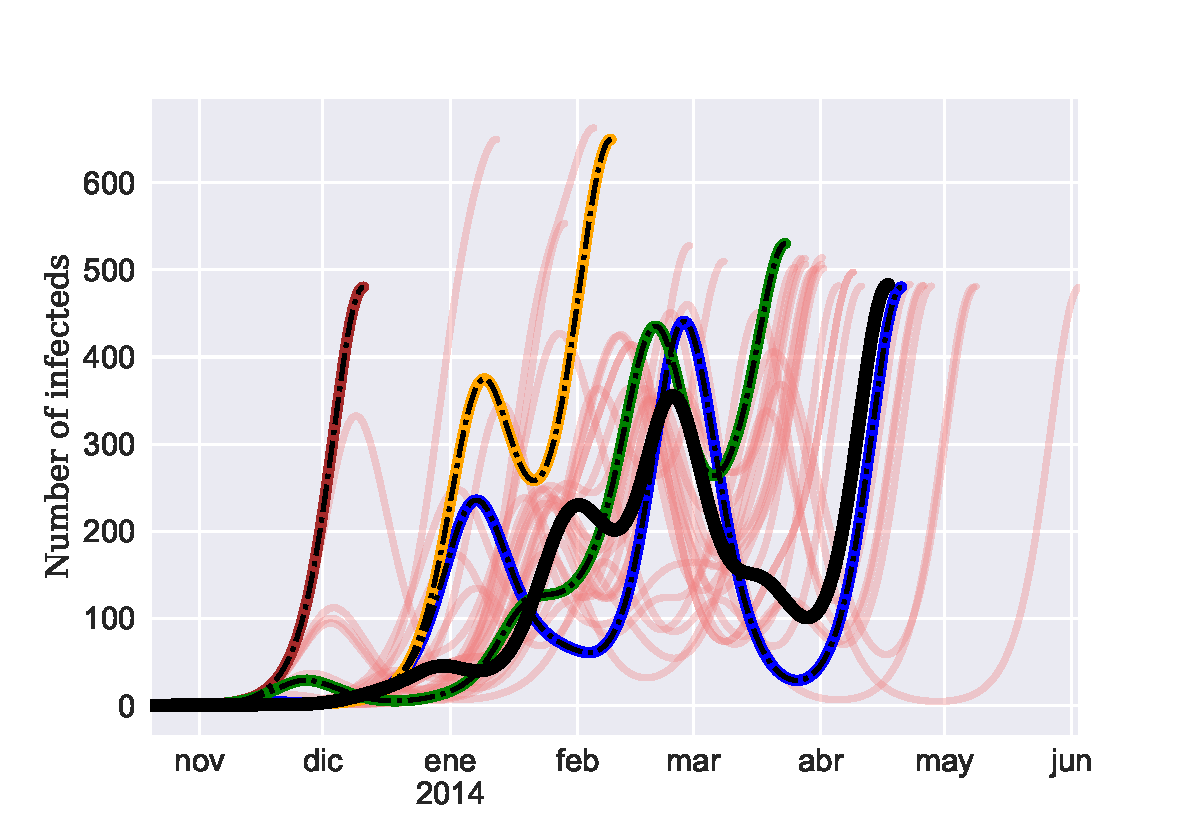
\includegraphics[scale=.45]{./scenario4_scenarioB-3}
%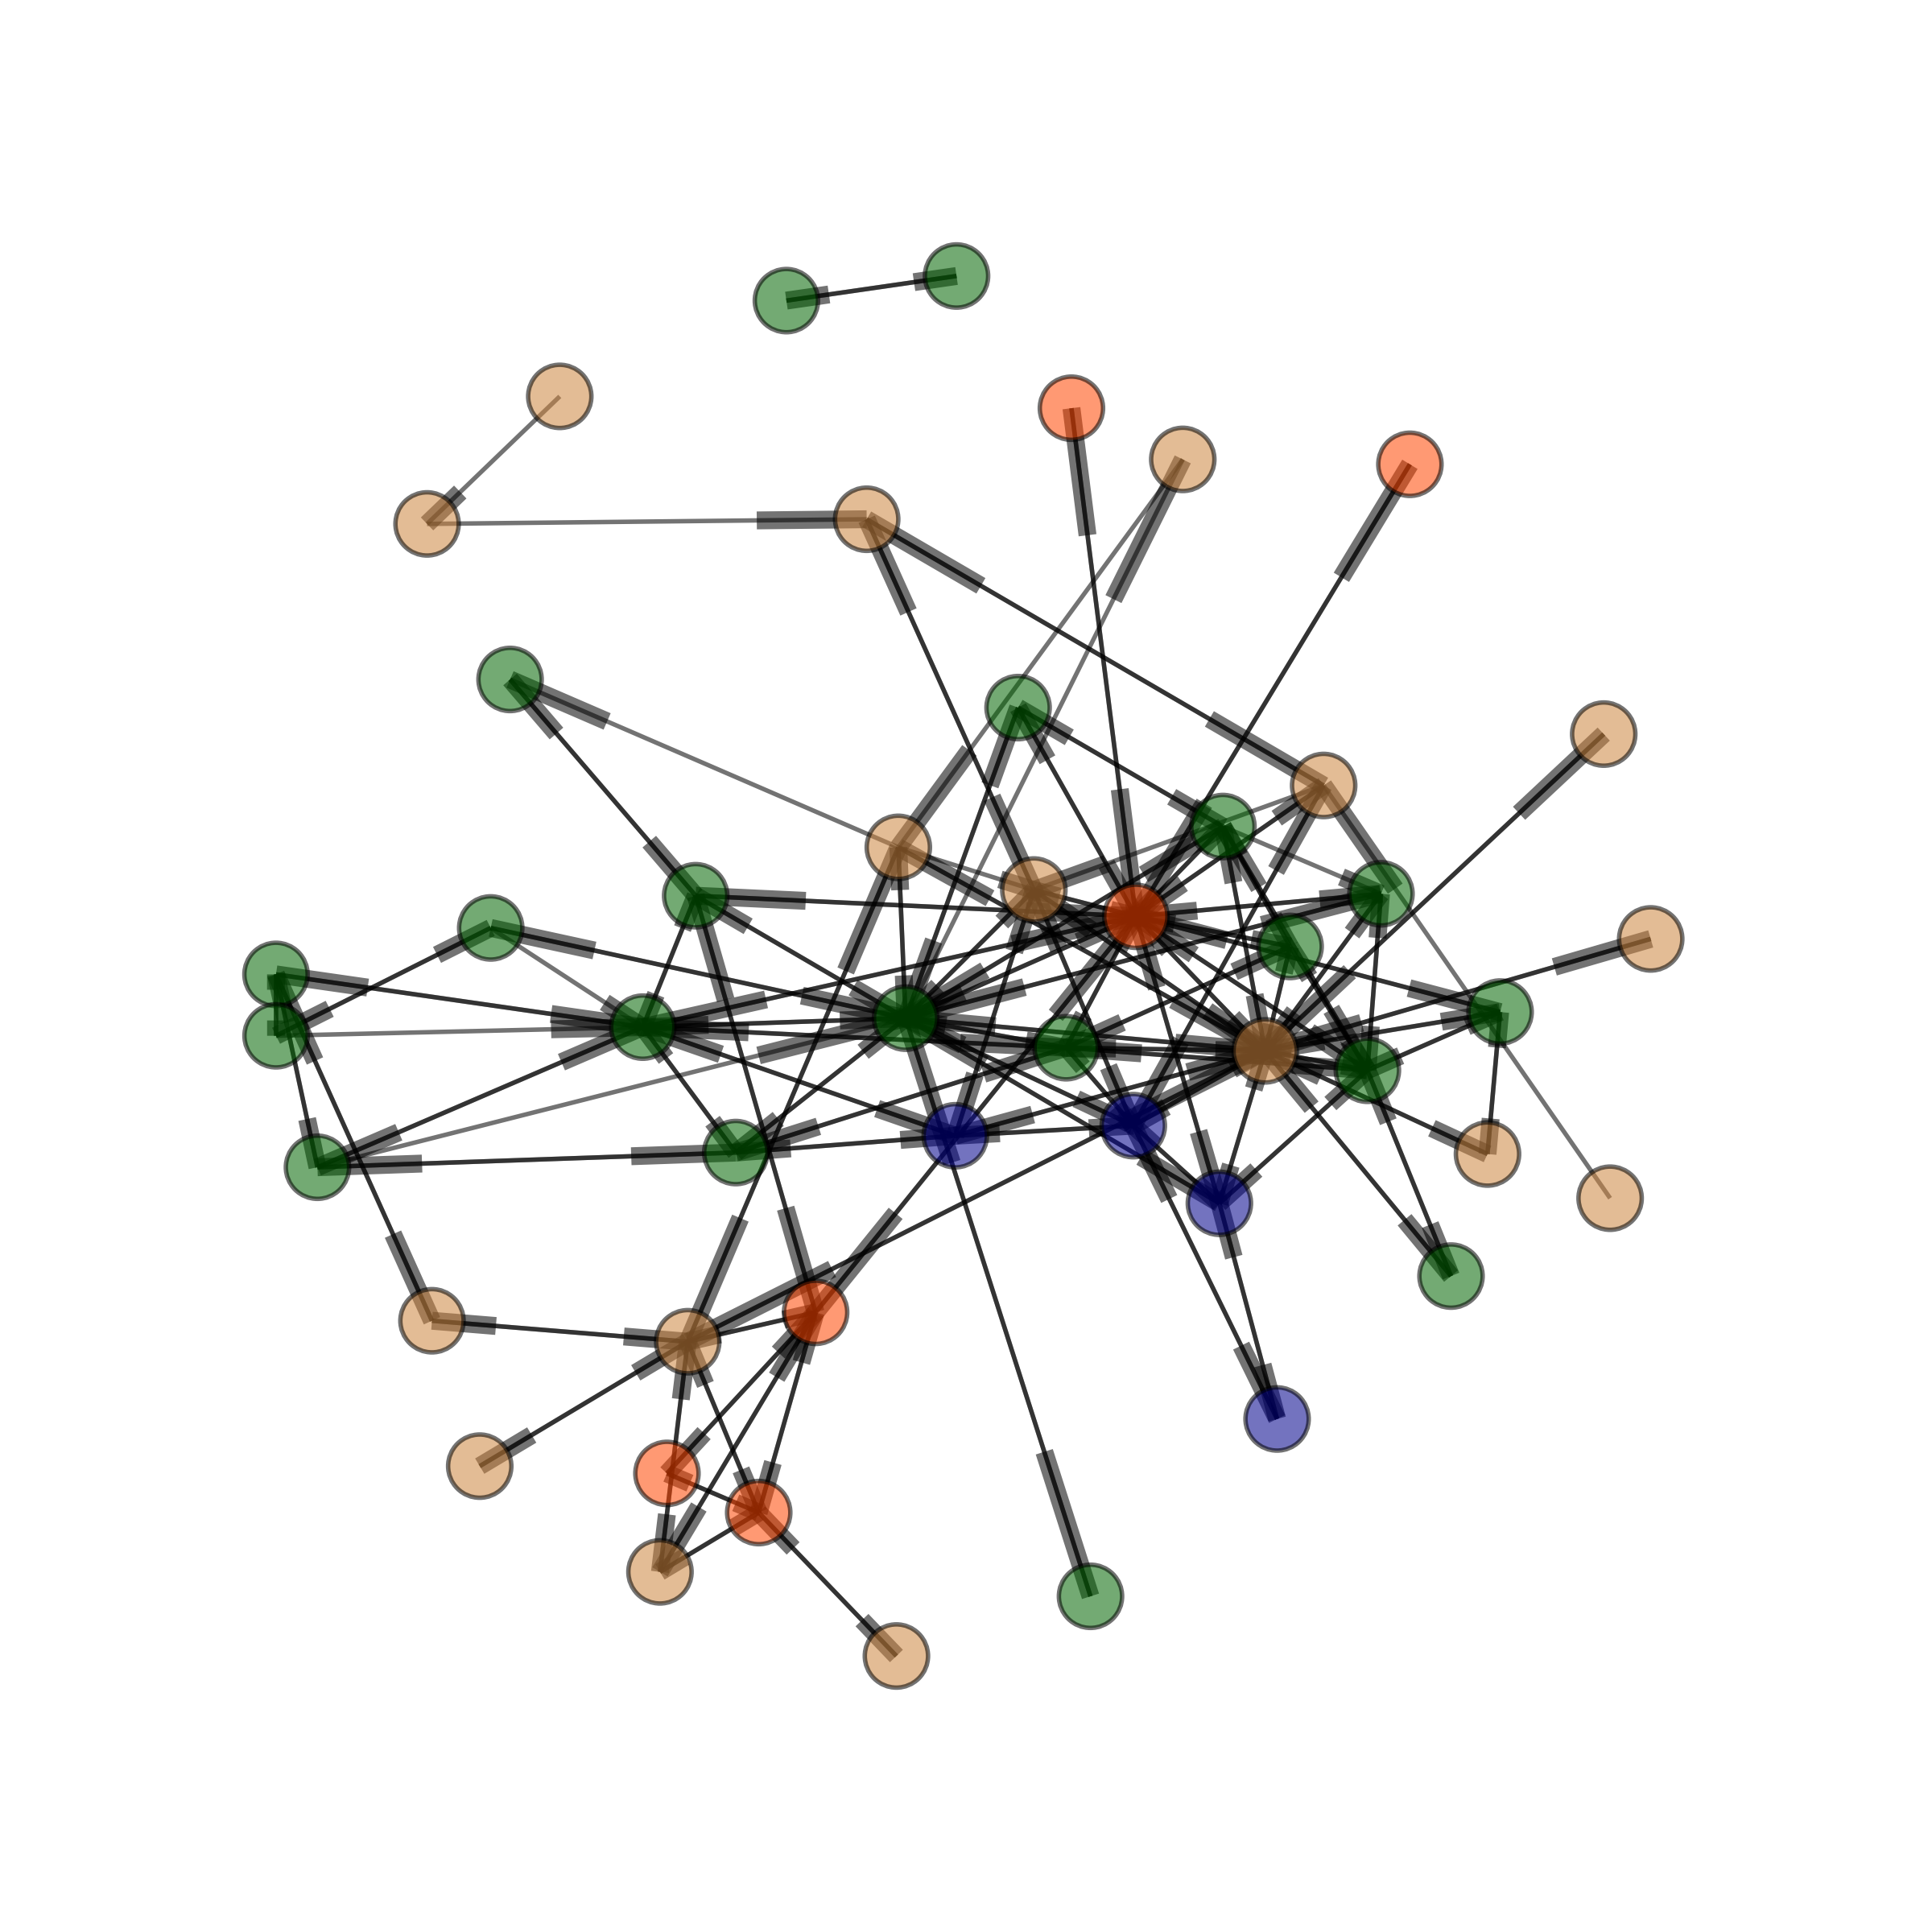
\includegraphics[scale=.30]{./graph_region3_colored}
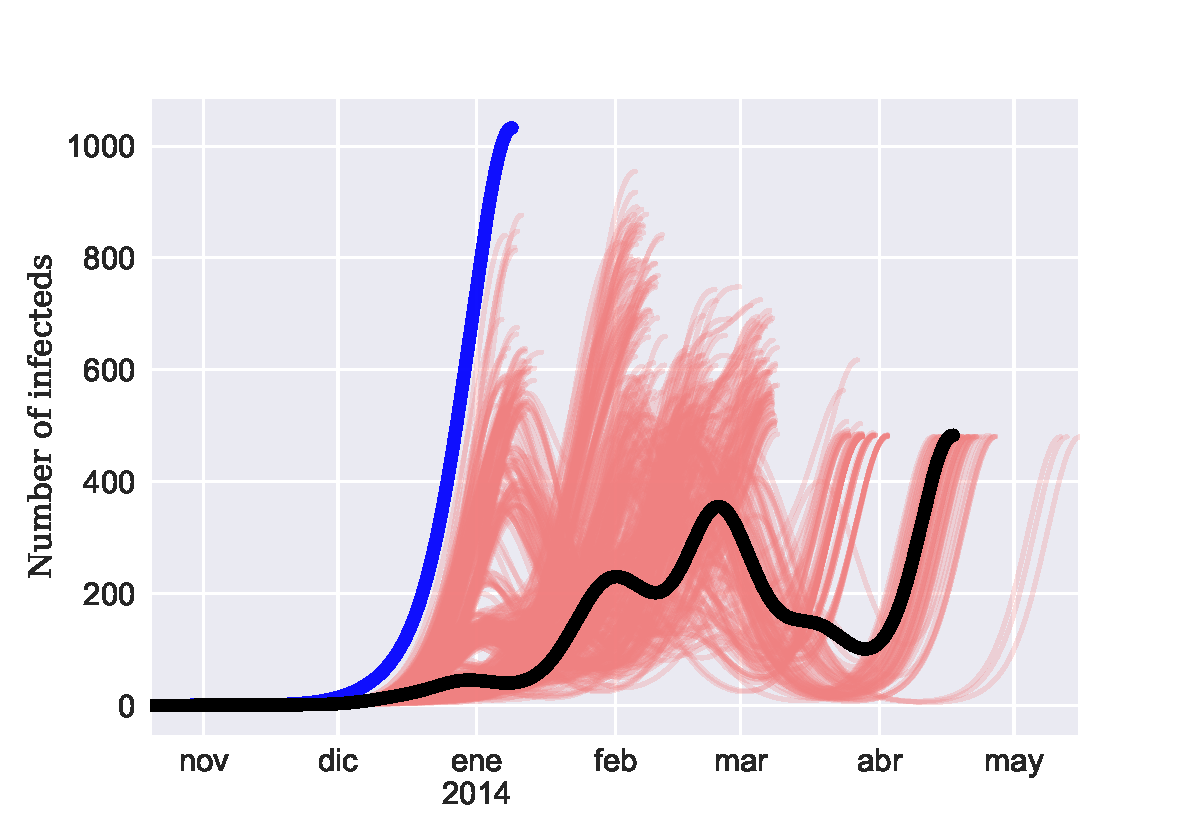
\includegraphics[scale=.30]{./scenario_A_2peak_2}
%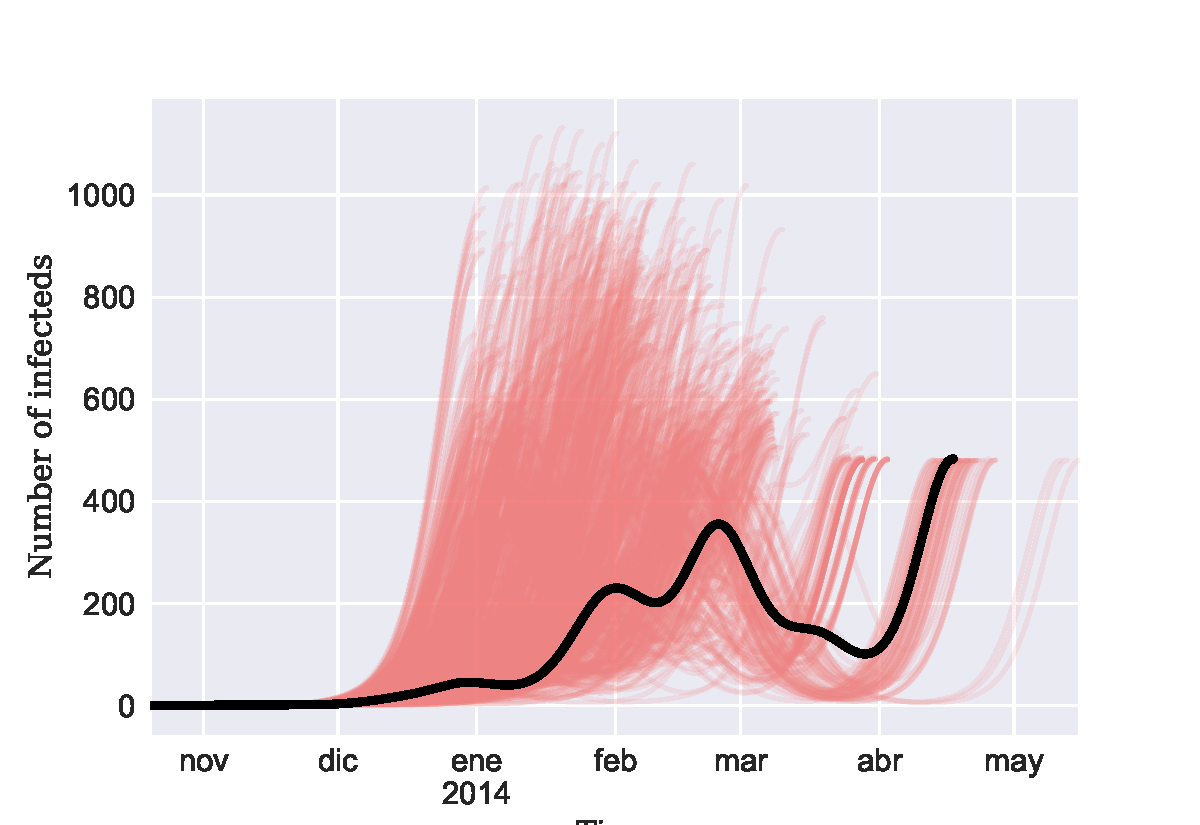
\includegraphics[scale=.30]{./scenario_D_2peak}
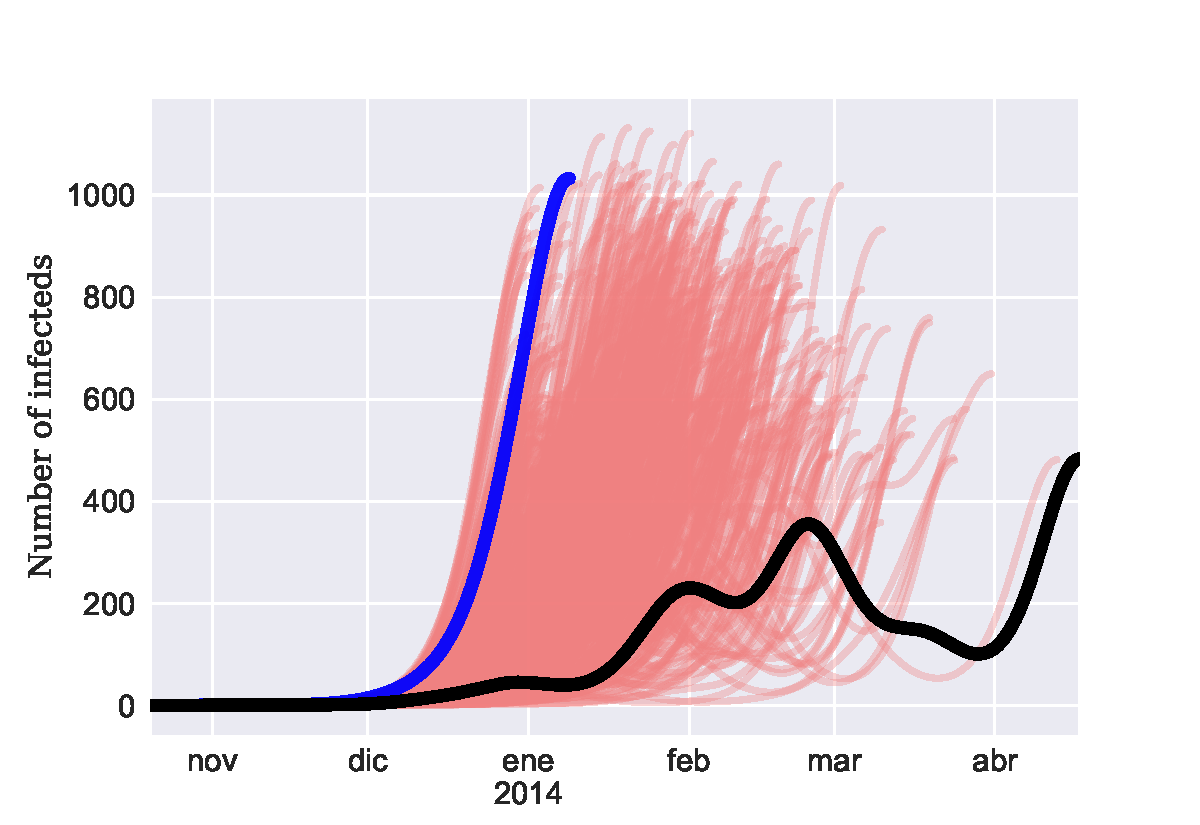
\includegraphics[scale=.30]{./scenario_ER_network_2}
\caption{\small Simulation scenarios. Top is the network model of airline connections and colors classify nodes regard official lnaguages spoken at each region: blue (French), orange (Ducth), latin-spanish(brown), and anglo/english (green). Top right are simulations (light red curves) of the fitted model where infection was initiated at each of the nodes of the network model other than in Saint Martin (which is represented by the solid black curve), the colored curves correspond to the outbreaks which start at the largest node population-wise of the nodes grouped by spoken language, which corresponding colors. Bottom left represent the scenario where the links for the initial Saint Martin have been randomized (light red); and bottom left represnt the scenario where the links for all nodes have been randomized following a Erd\"{o}-Renyi random network model (ligh red). The modeled outbreak initiated in Saint Martin is the black solid curve. The solid blue curves (bottom leaft and right) correspond to the homogeneous model where the initial infected island of Saint Martn ins connected to each other node locations of the network model}
\label{fig:scenarios}
\end{figure}
%
\vspace{2cm}
%
\begin{figure}[ht]
\centering
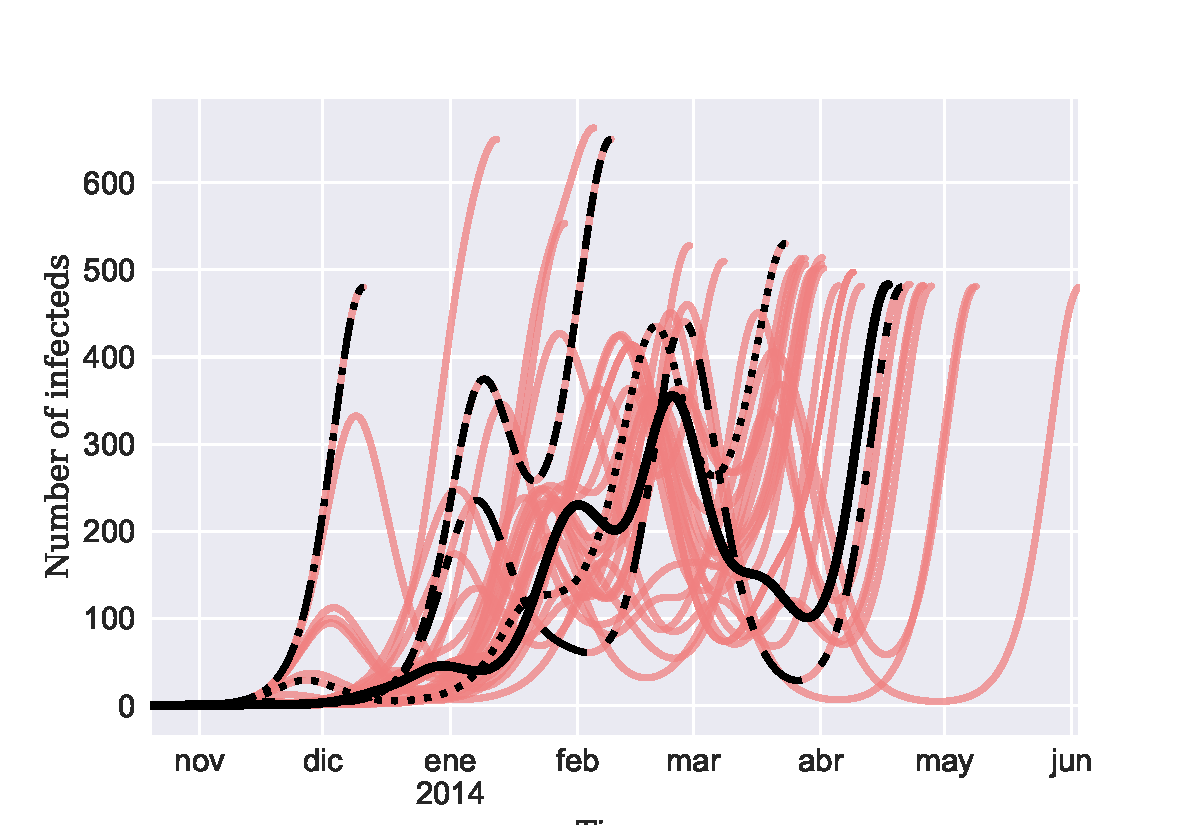
\includegraphics[scale=.45]{./scenario4_scenarioB-2}\\
%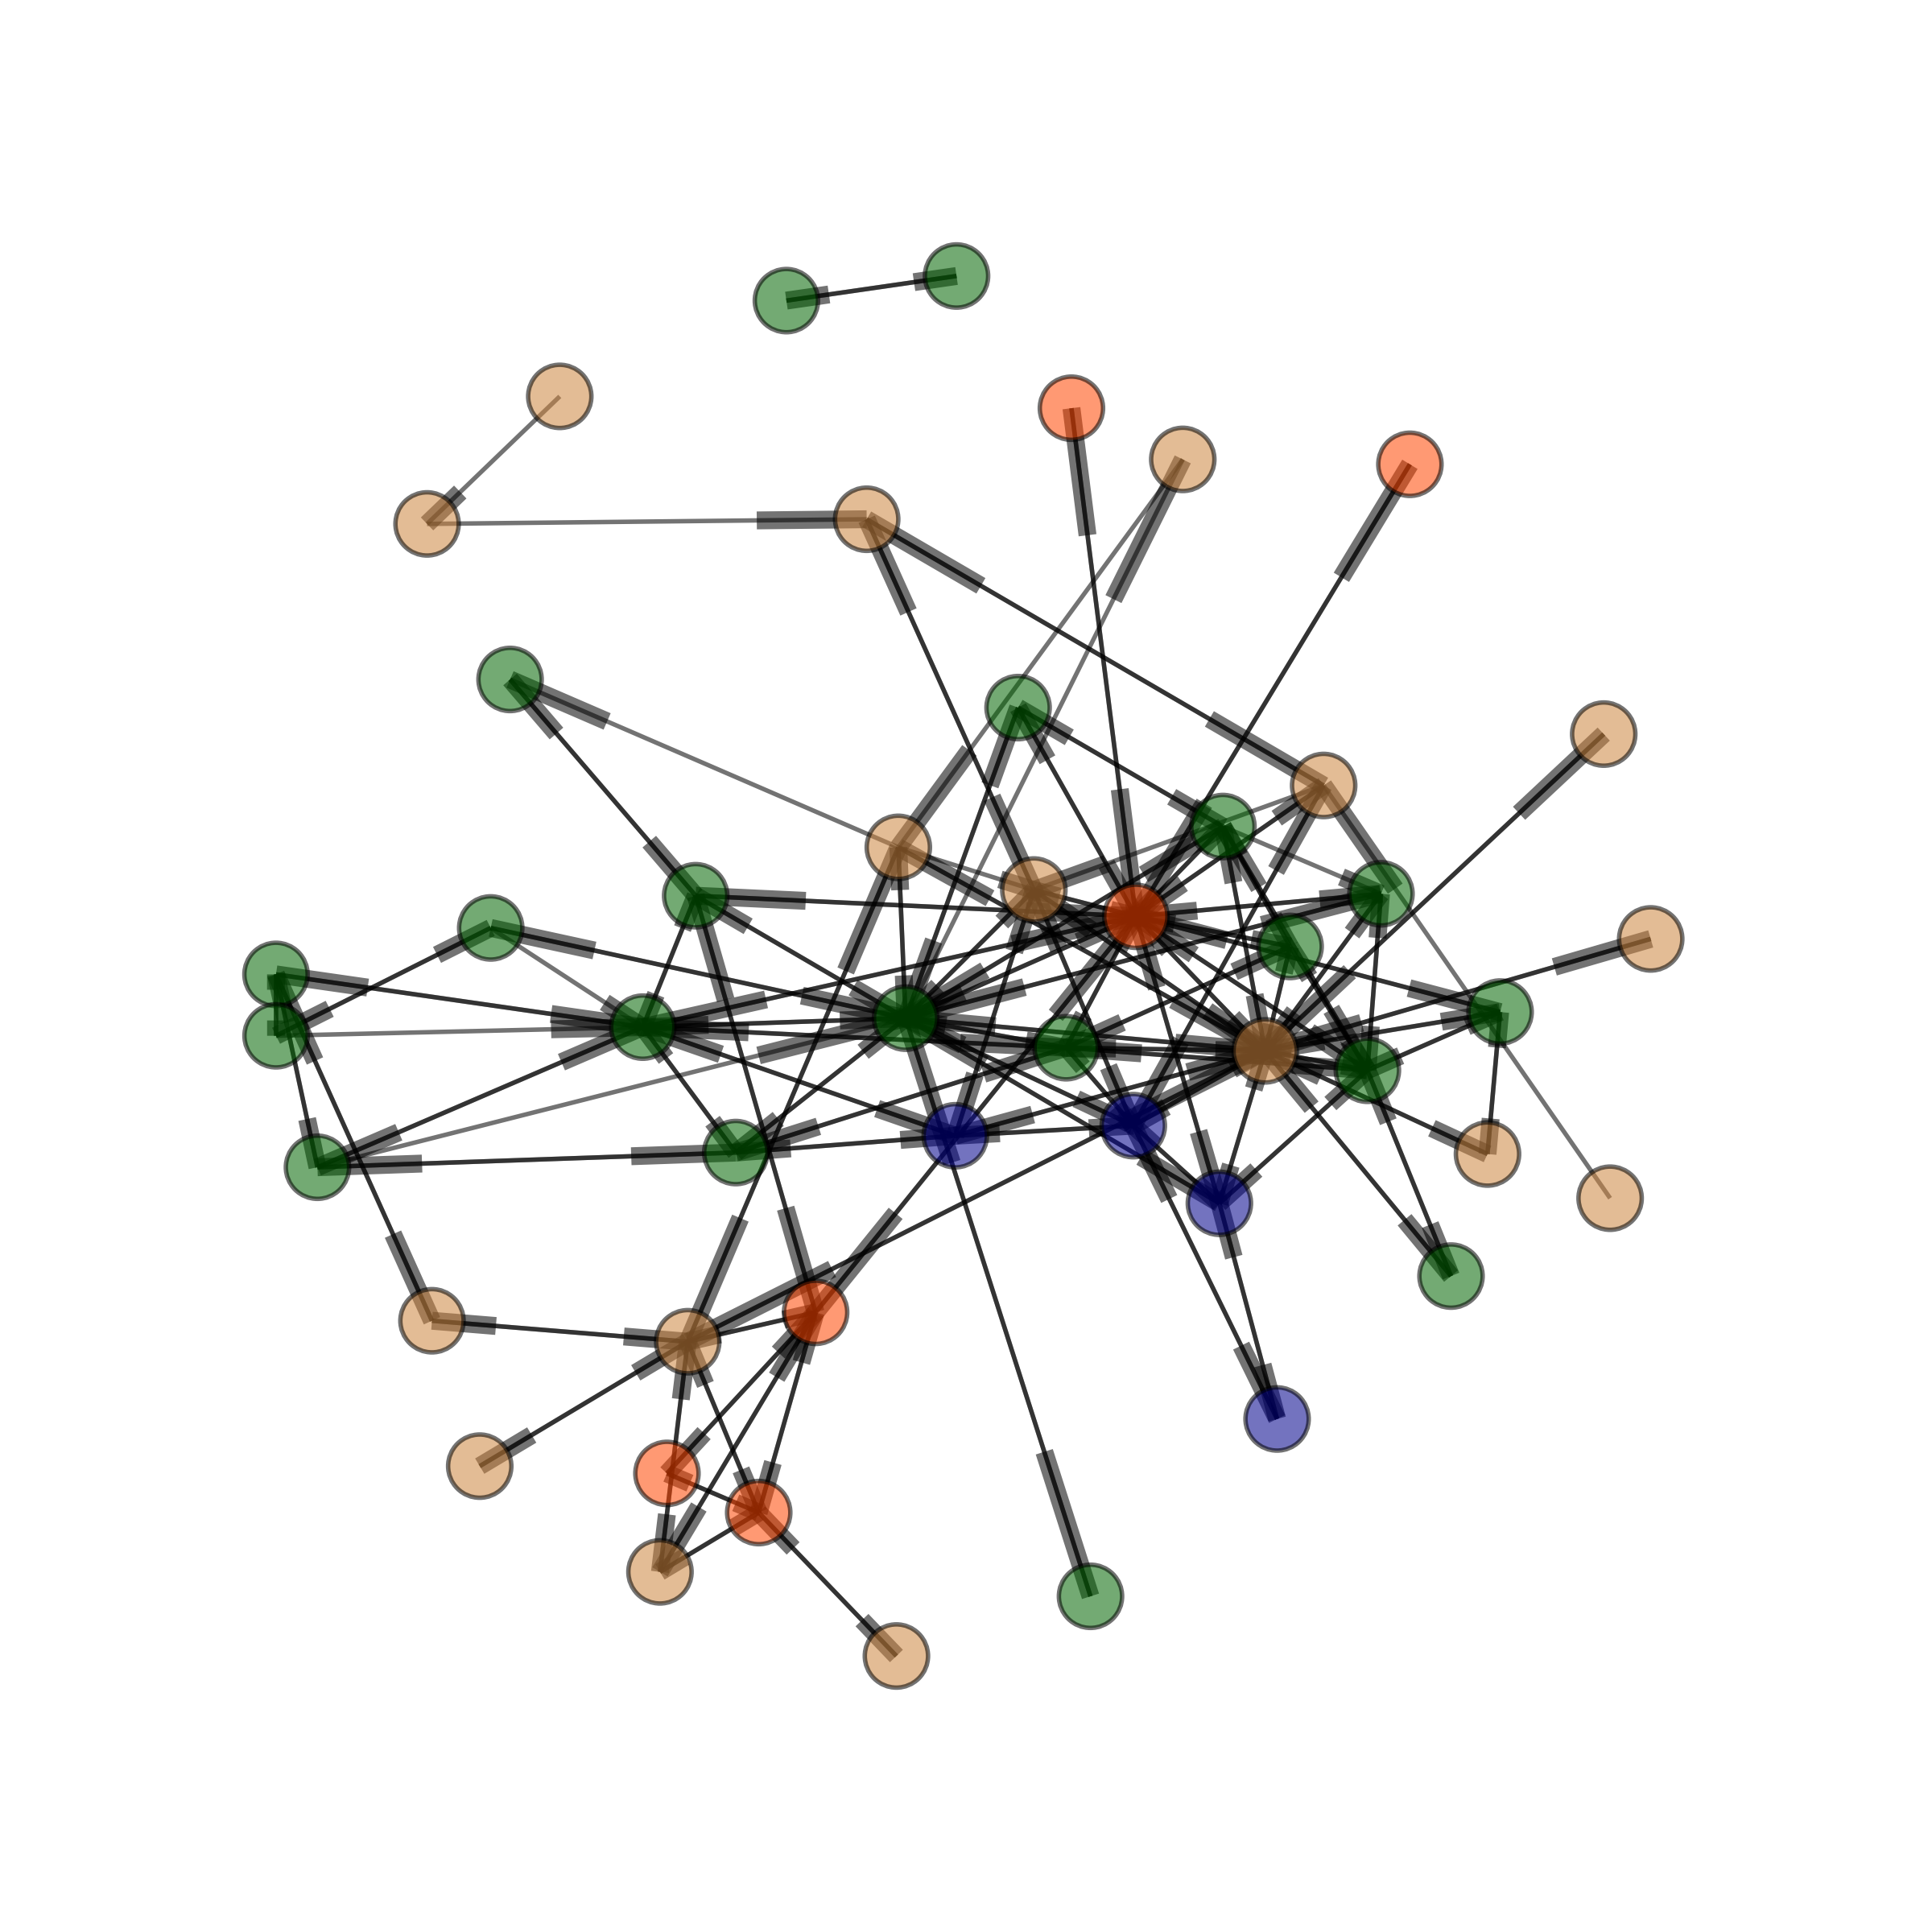
\includegraphics[scale=.30]{./graph_region3_colored}
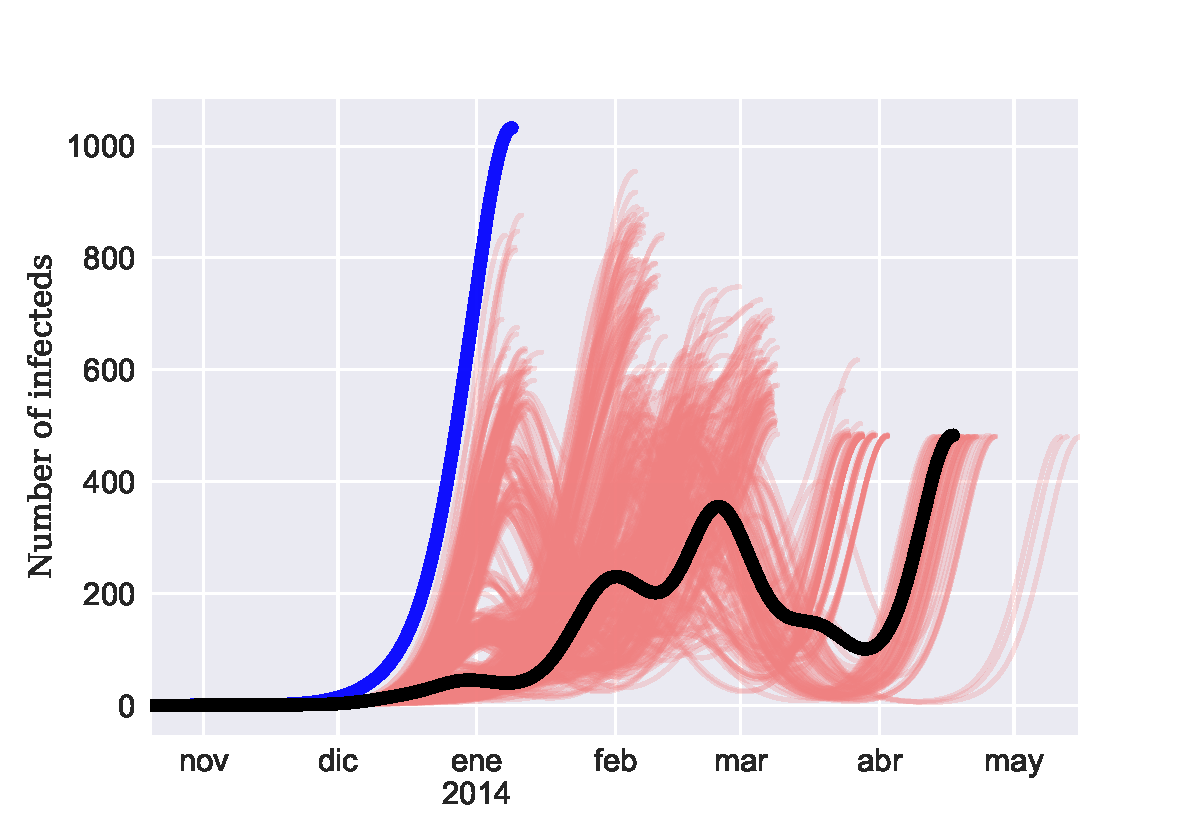
\includegraphics[scale=.30]{./scenario_A_2peak_2}
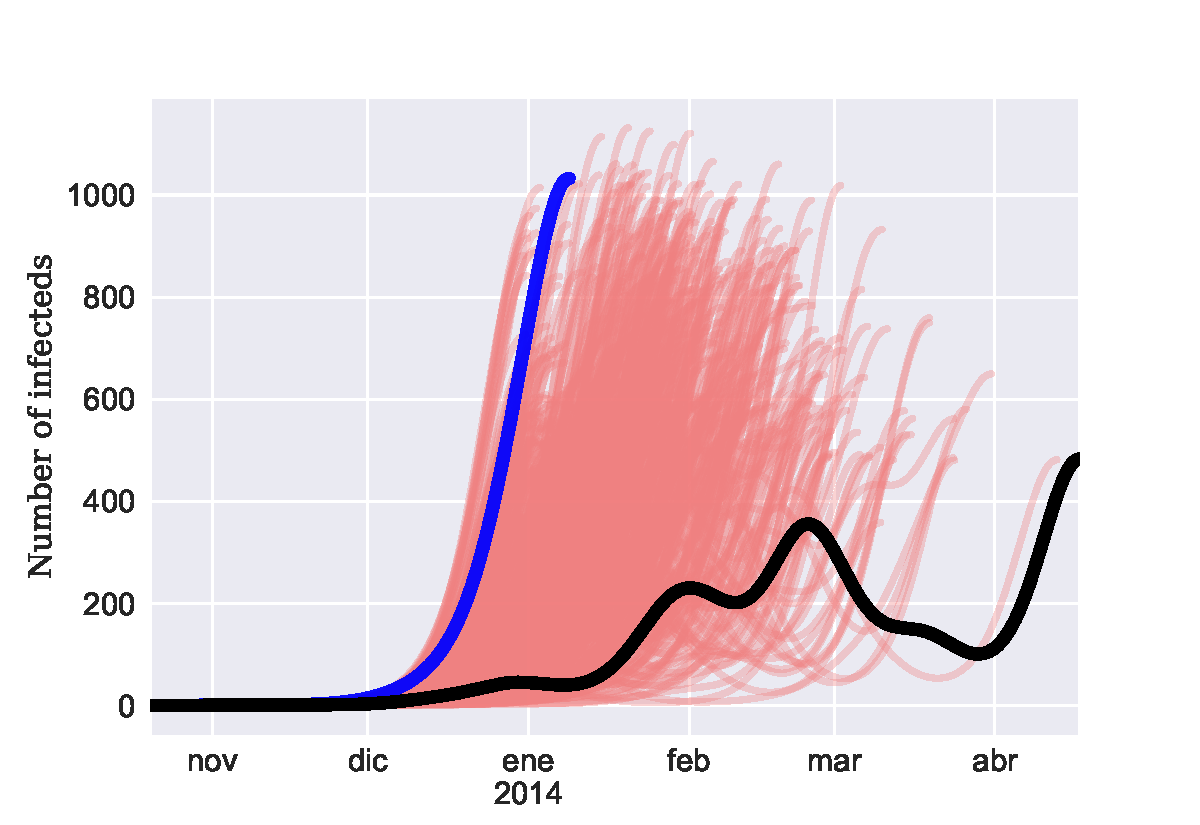
\includegraphics[scale=.30]{./scenario_ER_network_2}
\caption{\small Simulation scenarios (Alternative). Top is the network model of airline connections and colors classify nodes regard official lnaguages spoken at each region: blue (French), orange (Ducth), latin-spanish(brown), and anglo/english (green). Top right are simulations (light red curves) of the fitted model where infection was initiated at each of the nodes of the network model other than in Saint Martin (which is represented by the solid black curve), the colored curves correspond to the outbreaks which start at the largest node population-wise of the nodes grouped by spoken language, which corresponding colors. Bottom left represent the scenario where the links for the initial Saint Martin have been randomized (light red); and bottom left represnt the scenario where the links for all nodes have been randomized following a Erd\"{o}-Renyi random network model (ligh red). The modeled outbreak initiated in Saint Martin is the black solid curve. The solid blue curves (bottom leaft and right) correspond to the homogeneous model where the initial infected island of Saint Martn ins connected to each other node locations of the network model}
\label{fig:scenarios-alt}
\end{figure}
%
\vspace{2cm}
%
\begin{figure}[ht]
\centering
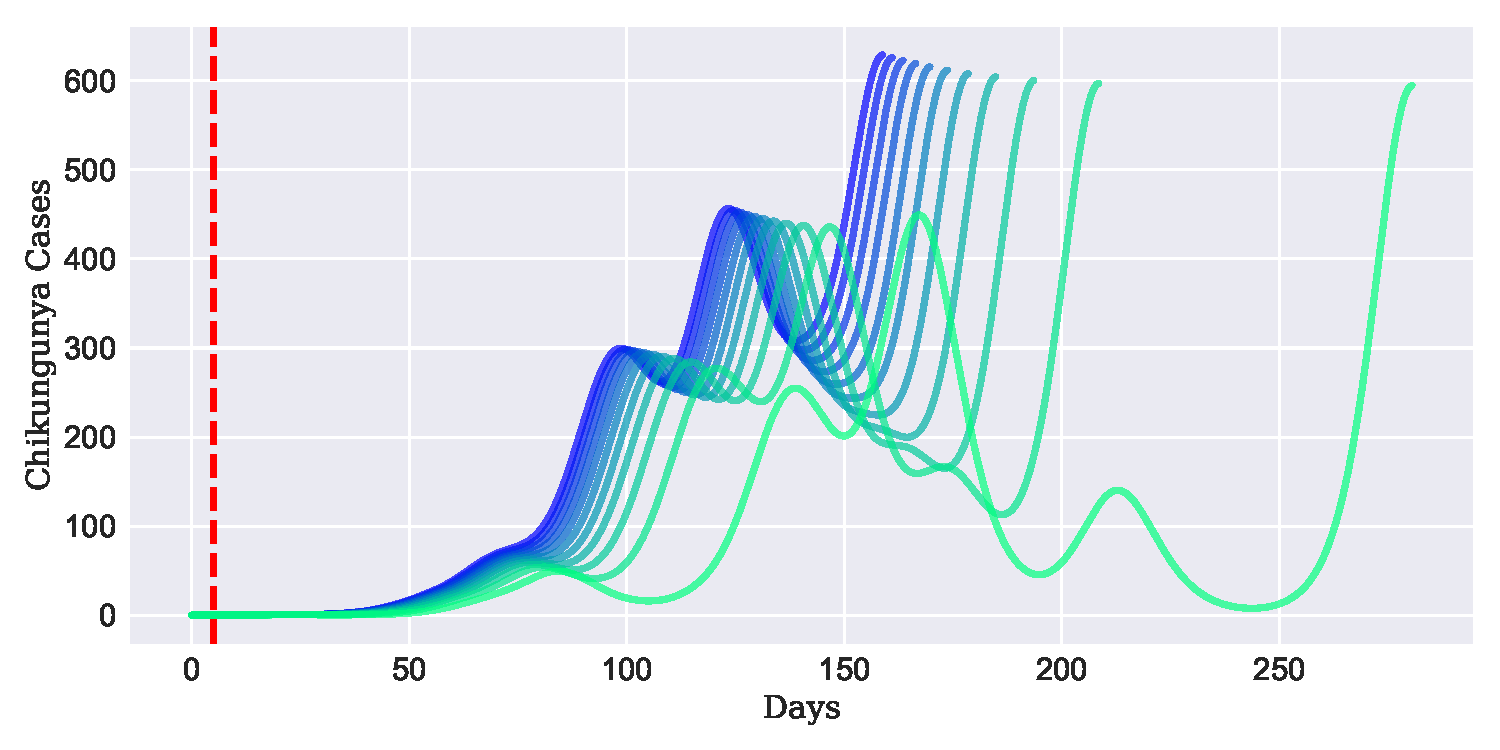
\includegraphics[scale=.24]{./interv_005}
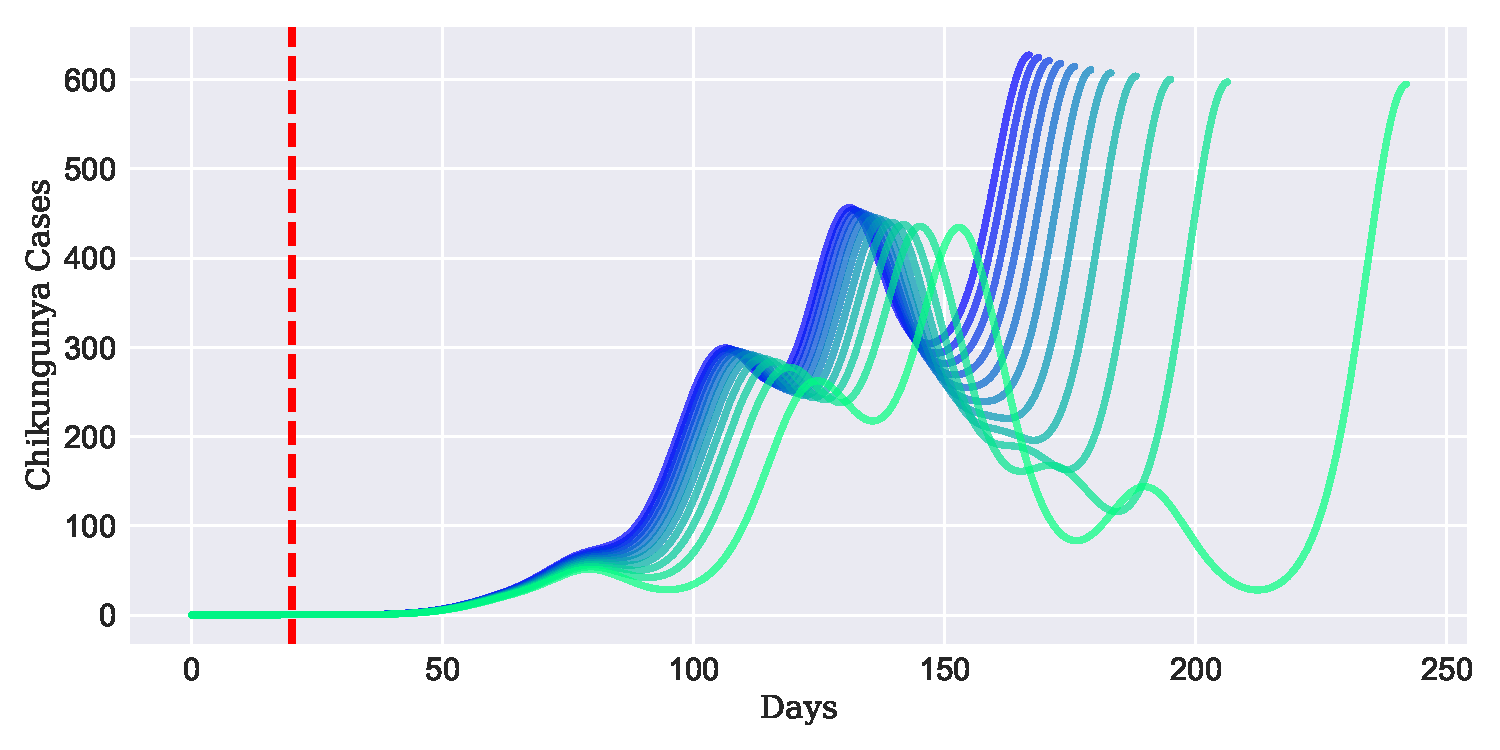
\includegraphics[scale=.24]{./interv_020} \\
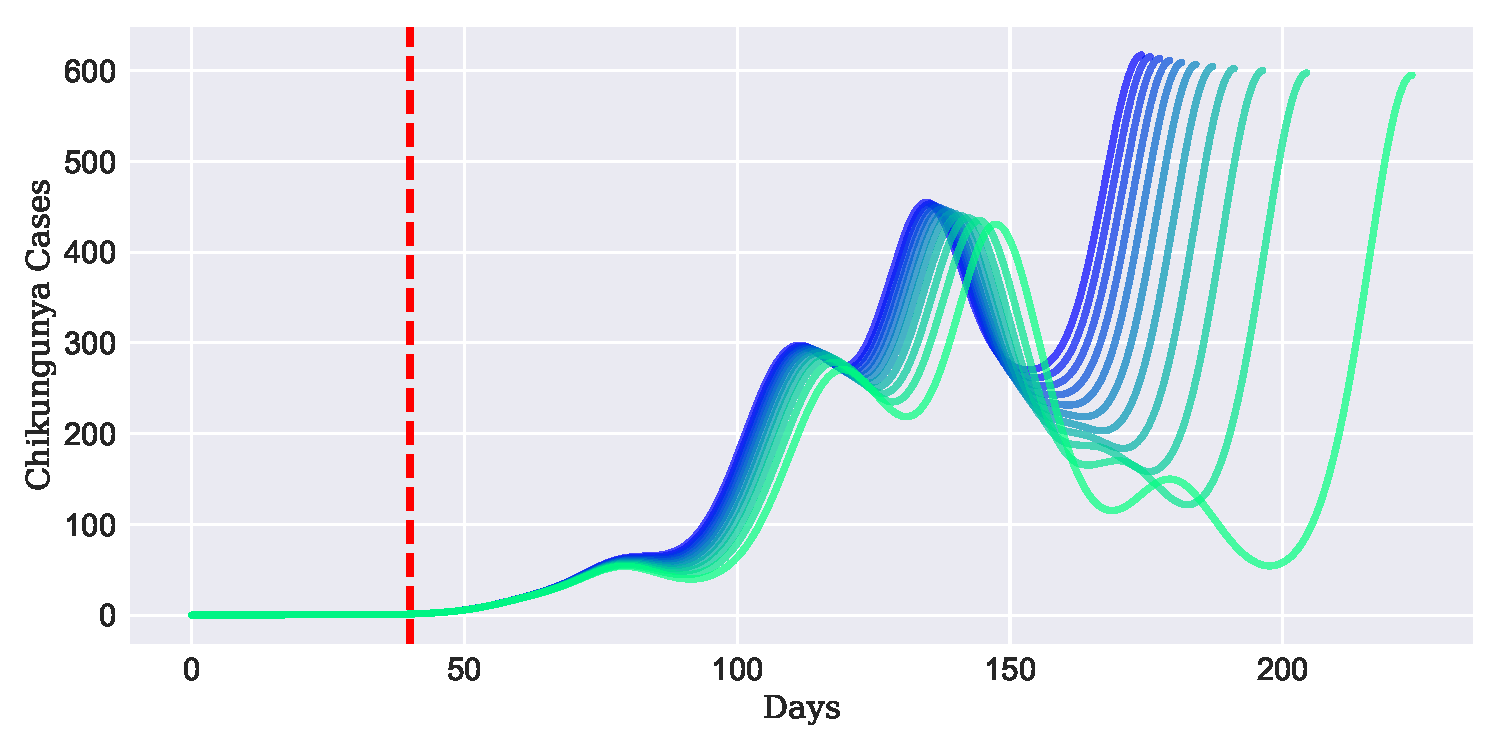
\includegraphics[scale=.24]{./interv_040}
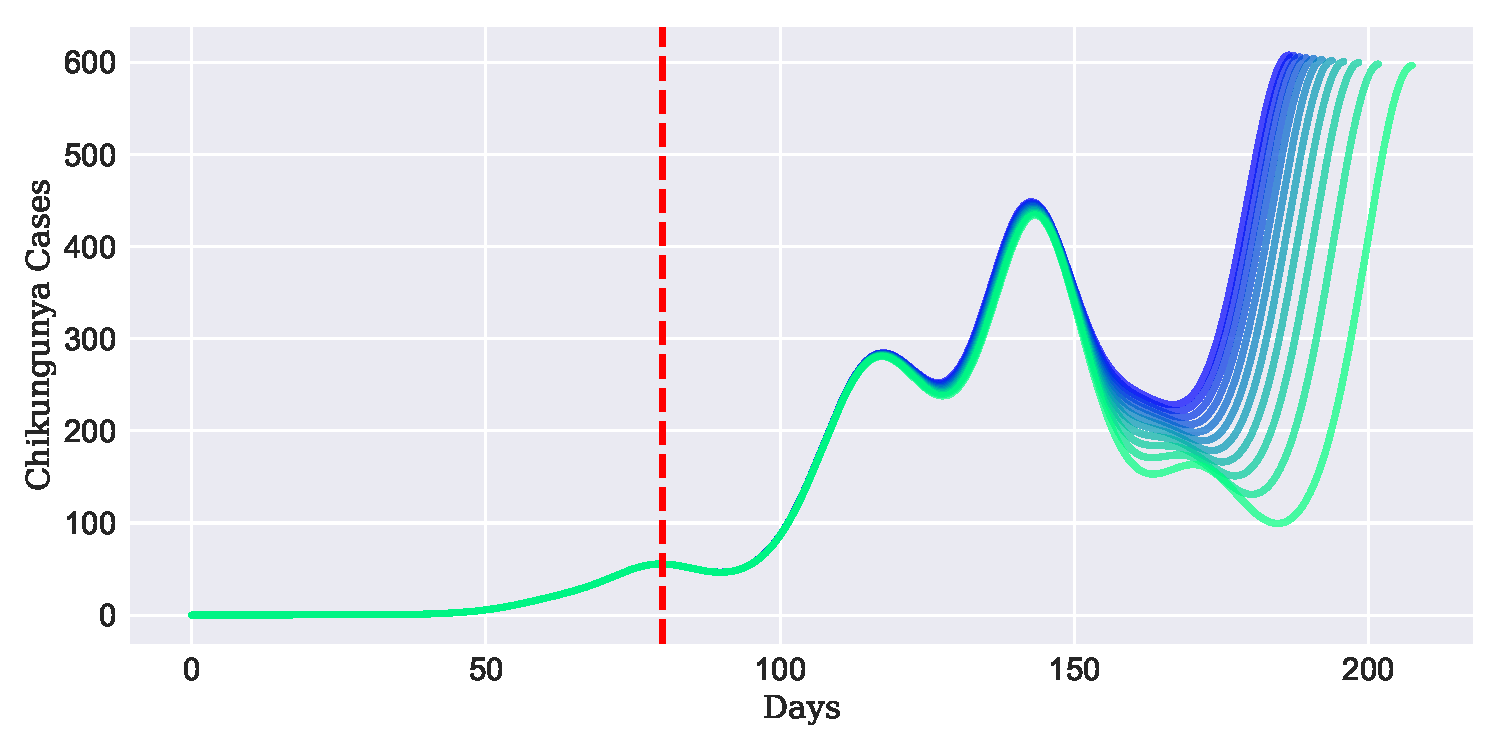
\includegraphics[scale=.24]{./interv_080} \\
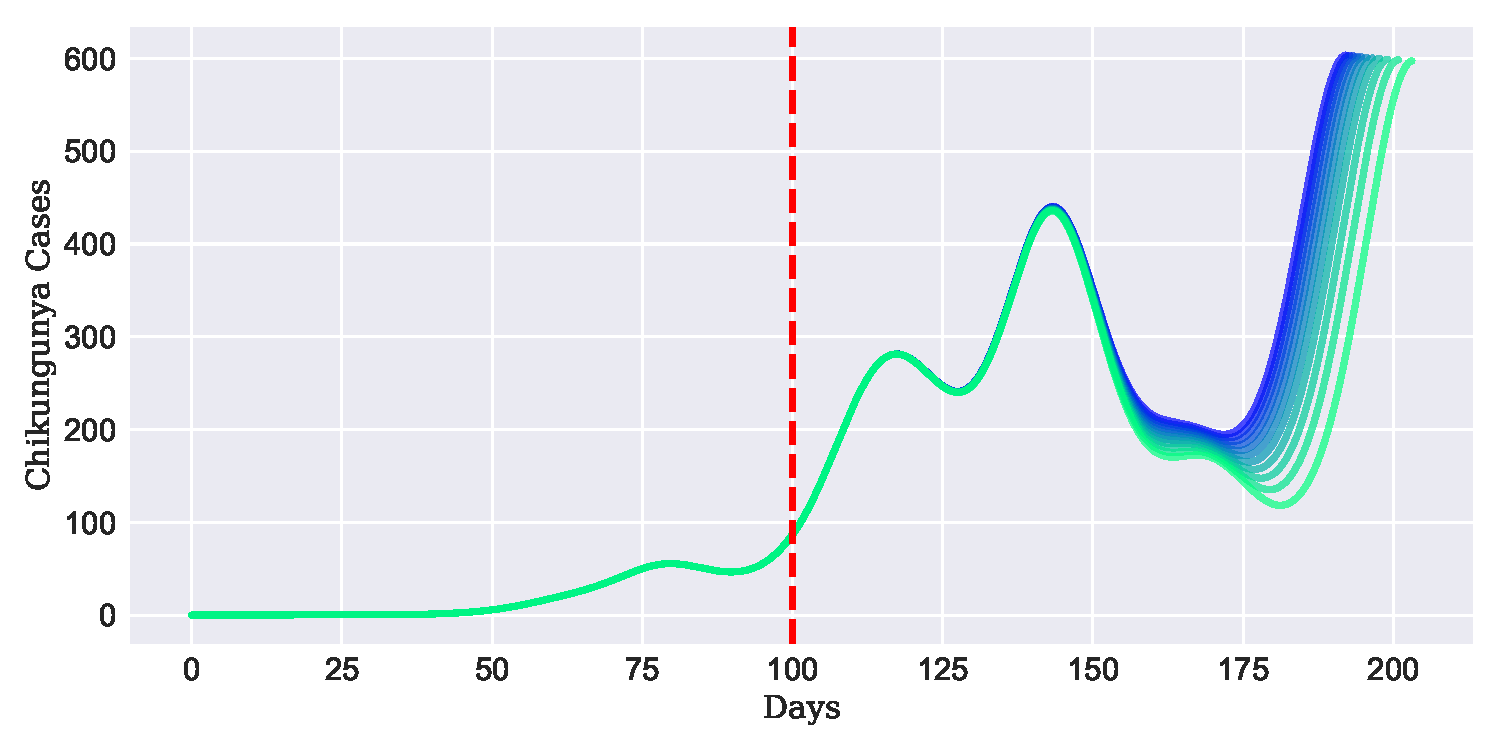
\includegraphics[scale=.24]{./interv_100}
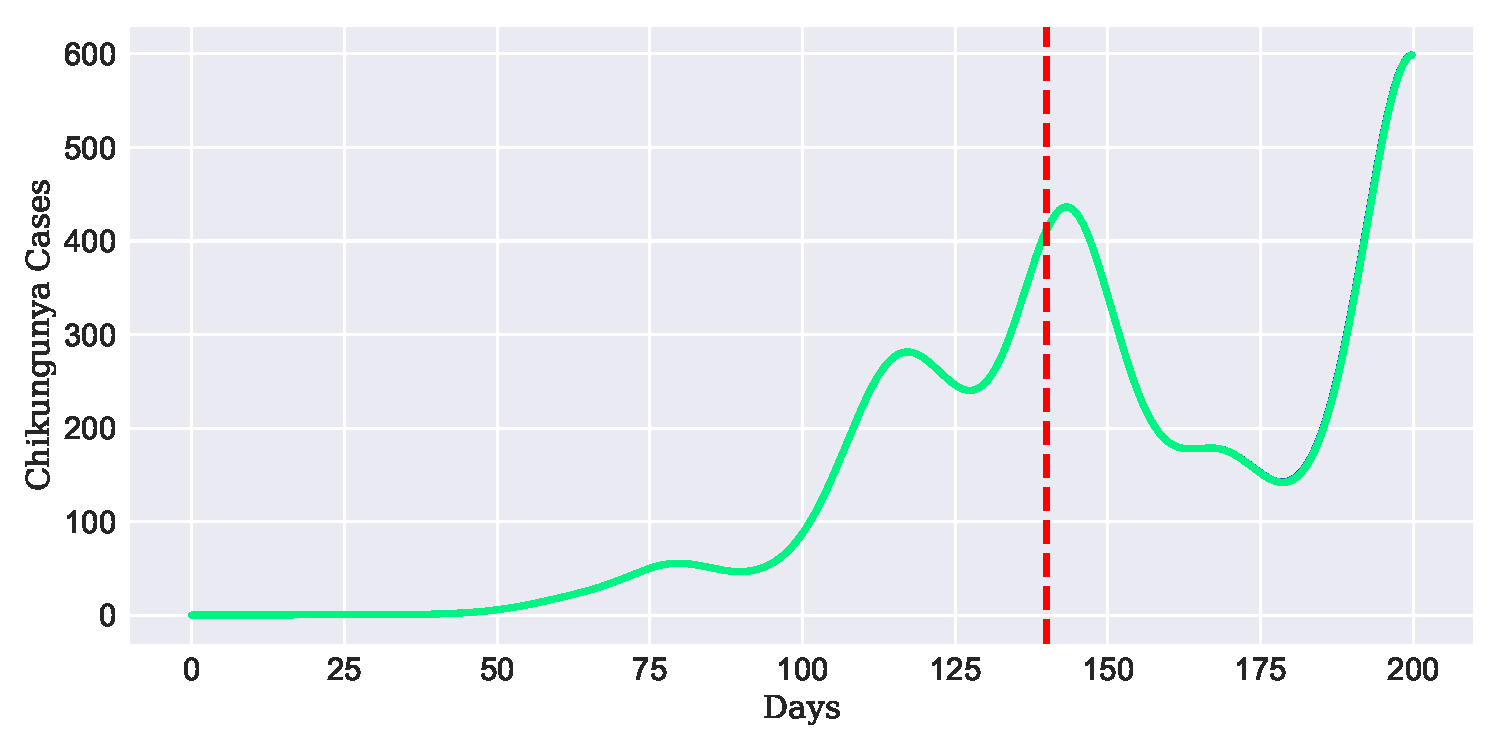
\includegraphics[scale=.24]{./interv_140}
\caption{\small . Intervention scenarios. Level of reductions of air  traffic have been perfomed on the fitted network model to assess epidemic severity under control scenarios. Ten reduction levels were performed: from 100\% (total cut off air traffic), 90\%, ..., up to 0 \% (not cut off at all). Simulations of the network model were executed with these interventions and outbreak curves were plotted. The more blue indicates higher level of intervention (higher cut off of the air traffic). The vertical red line indicate the time when the interventions were made.}
\label{fig:interventions}
\end{figure}
\vspace{5cm}
%
\begin{figure}[ht]
\centering
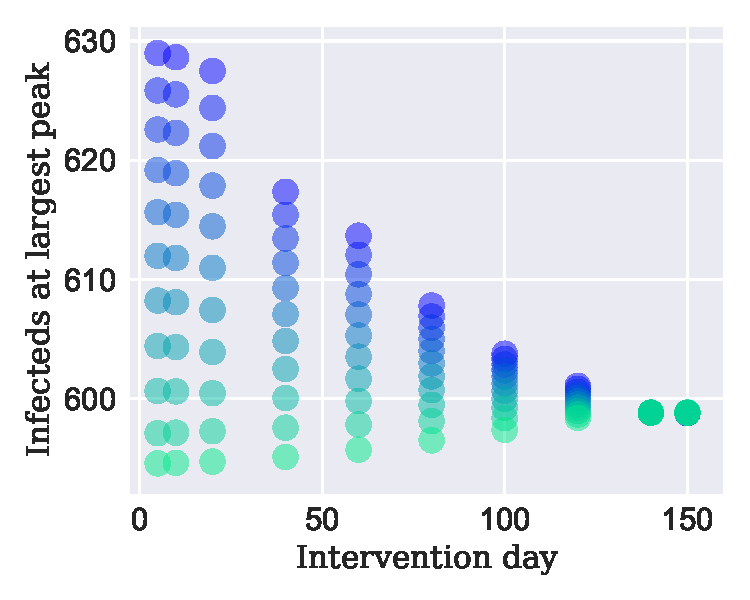
\includegraphics[scale=.32]{./intervention_summary_A}
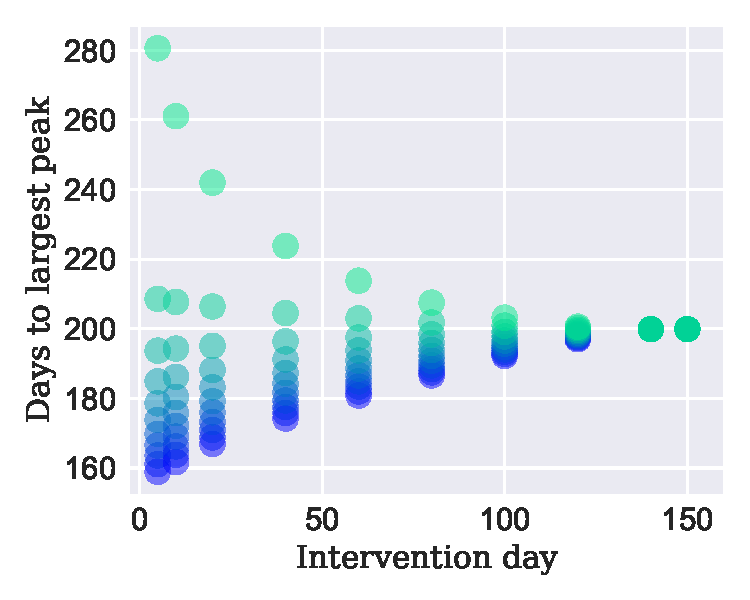
\includegraphics[scale=.32]{./intervention_summary_B}
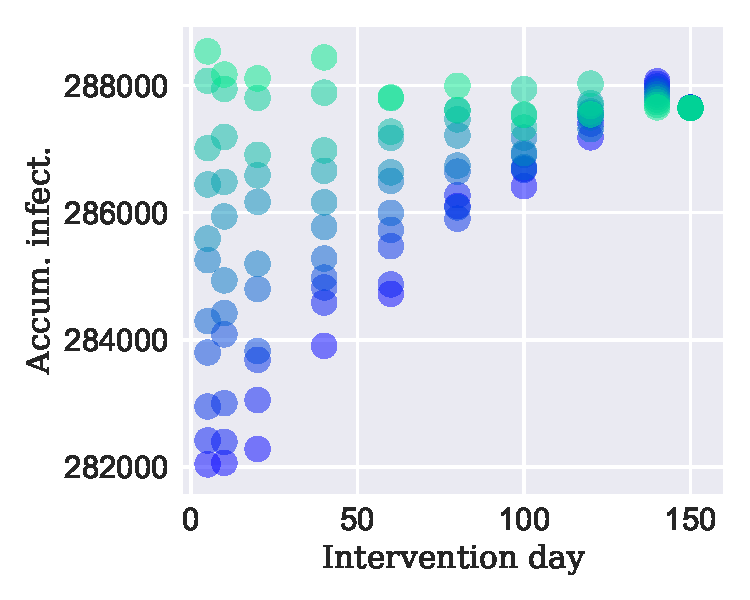
\includegraphics[scale=.32]{./intervention_summary_C}
\caption{\small Intervention scenarios. Right plot indicates the edpidemic severy as a function of both the day of intervention since the epidemic day zero (in the x-axis) and the level of intervention (indicate by the intensity of blue- the more blue the largest the intervention the more green the less intervention). The plot of the right measures the epidemic severity as the number of infected individuals at the maximum epidemic peak, the plot in the center measures the epidemic severity as the number of days to the maximum epidemic peak, and the plot of the left measures epidemic severy as the number of accumulated infected individuals at the maximum epidemic peak.  
}
\label{fig:interventions-summary}
\end{figure}

%
\begin{table}[ht]
\centering
\begin{tabular}{|c|c|c|}
\hline
\textbf{Parameter} & \textbf{Definition} & \textbf{Fitted Value} \\
\hline
$\beta$ & Transmission rate & 1.21 day$^{-1}$ \\
\hline
$\sigma$ & Incubation period & 0.35 day$^{-1}$\\
\hline
$\gamma$ & Recovery rate & 0.57 day$^{-1}$\\
\hline
\end{tabular}
\caption{\label{tab:parameters} \small Parameters of the epidemic model estimated by least squares form the observed incidence series.}
\end{table}

\begin{center}
    \begin{tabular}{| c | p{3cm} | p{3cm}| p{3cm} |}
    \hline
    Scenario & Infecteds at Peak (mean/sd)& Time to Peak (days mean/sd) & Accumulated Infecteds at peak (mean/sd) \\ \hline
    Scenario 1 & 577.2/104.1  & 129.6/30.2 & 363192.2/133459.7 \\ \hline
    Scenario 2 & 1032.4/0.0 * & 80.0/0.0 *  & 338688.1/0.0 * \\ \hline
    Scenario 3 & 734.8/166.6 & 103.1/18.6 & 327661.9/97152.9 \\ \hline
    Scenario 4 & 497.2/104.9 & 152.8/44.0 & 439021.1/129005.4 \\
    \hline
    \end{tabular}
    {\small Table 2: Epidemic scenarios summary.}
    \ref{table:scenarios}
%    \caption{\small Sscenario summary.}
\end{center}

\end{document}
